\documentclass{article}

% Language setting
% Replace `english' with e.g. `spanish' to change the document language
\usepackage[english]{babel}
\usepackage{caption}
% Set page size and margins
% Replace `letterpaper' with`a4paper' for UK/EU standard size
\usepackage[letterpaper,top=2cm,bottom=2cm,left=3cm,right=3cm,marginparwidth=1.75cm]{geometry}

% Useful packages
\usepackage{amsmath}
\usepackage{graphicx}
\usepackage{authblk} % this is for multiple autho  rs 
\usepackage[colorlinks=true, allcolors=blue]{hyperref}
\usepackage{cleveref}
\usepackage{booktabs}
\usepackage{multirow}

% Configure for "Fig.":
\crefname{figure}{Fig.}{Figs.}
\Crefname{figure}{Fig.}{Figs.}


% reference configuration
\usepackage[authoryear,round]{natbib}
\bibliographystyle{apalike} % for an APA-like style
\usepackage{amsmath}

%%%%%%%%%%%%%%%%%%%%%%%%%%%%%%%%%%%%
%%% --- Tittle of the paper --- %%%
%%%%%%%%%%%%%%%%%%%%%%%%%%%%%%%%%%
\title{\textbf{Development of outdoor air pollution models for estimating exposure in the Barcelona Life Study Cohort (BiSC)}}

%%%%%%%%%%%%%%%%%%%%%%%%%%%%%%%%%%%%%%%%%
%%% --- Authors and affiliations --- %%%
%%%%%%%%%%%%%%%%%%%%%%%%%%%%%%%%%%%%%%%

%%% --- Authors --- %%%
\author[1, 2, 3]{Alan Domínguez}
\author[1, 3, 4]{Payam Dadvand}
\author[1]{Marta Cirach}
\author[1]{Bruno Raimbault}
\author[1]{Toni Galmes}
\author[1]{Karl Samuelsson}
\author[1, 2, 3]{Mark Nieuwenhuijsen}
\author[1, 2, 3]{Jordi Sunyer}
\author[1, 2, 3]{Xavier Basagaña}
\author[1, 3]{Ioar Rivas}

%%% --- Affiliations --- %%%
\affil[1]{Barcelona Institute for Global Health (ISGlobal), Barcelona, Spain.}
\affil[2]{Universitat Pompeu Fabra (UPF), Barcelona, Spain.}
\affil[3]{CIBER Epidemiología y Salud Pública (CIBERESP), Madrid, Spain.}
\affil[4]{London School of Hygiene and Tropical Medicine (LSHTM), London, UK.}

%%%%%%%%%%%%%%%%%%%%%%%%%%%%%%%%%%%%%%%%%%%%%%%%%%%%%%%%%%%%%%%%%%%%%%%%%

\begin{document}
\maketitle

%%%%%%%%%%%%%%%%%%%%%%%%%
%%% --- Abstract --- %%%
%%%%%%%%%%%%%%%%%%%%%%%
\begin{abstract}

Air pollution is the leading environmental risk factor for human health worldwide linked to wide range of adverse health outcomes. A detailed and comprehensive exposure assessment of outdoor air pollution considering both spatial and temporal variability is fundamental to conduct epidemiological studies.  

\end{abstract}

%%%%%%%%%%%%%%%%%%%%%%%%%%%%%
%%% --- Introduction --- %%%%%%%%%%%%%%%%%%%%%%%%%%%%%%%%%%%%%%%%%
%%%%%%%%%%%%%%%%%%%%%%%%%%%
\section{Introduction}

Air pollution stands as the primary environmental risk factor for human health and the fourth most deadly health risk worldwide, playing a significant role in the global burden of disease \cite{cohen2017, he2020state}. Exposure to ambient air pollution has been linked with a extensive array of adverse health outcomes \cite{boogaard2022, guxens2022hei, haddad2023}. In this context urbanization have been playing a major role increasing air pollution exposure as cities grow and more population moves to urban areas \cite{nieuwenhuijsen2016}. This trends present challenges for epidemiological studies \cite{tonne2017}, where accurate estimates capturing both the spatial and temporal variability are essential to evaluate the health impacts of air pollution in urban areas \cite{boogaard2022}. 

Over the past few decades, several modelling techniques have been adopted in environmental epidemiology to determine exposure concentrations of air pollution \cite{hoek2017, di2019no2, di2019pm25, stafoggia2019, stafoggia2020}. Among these, Land use regression (LUR) and dispersion models (DM) are the most common approaches for estimating air pollution exposure concentrations in epidemiological studies \cite{gulliver2015, dehoogh2014}. LUR models employ regression techniques to predict air pollution levels at non-monitored locations, drawing on observed air pollution data and spatial explanatory variables that work as proxies for traffic-related air pollution \cite{briggs1997, hoek2008}. In contrast, DMs rely on mathematical simulations to estimate air pollution levels. These predictions are based on data from emissions sources, chemical transformation models, pollutant dispersion models, topography, roughness, and meteorological data \cite{hoek2017}. Although these methods have been extensively used they come with inherent limitations related to lack of temporal and spatial variation. To overcome the shortcomings, hybrid models (HM) have emerged, blending both spatial and temporal advantages, leading to refined and enhanced estimations \cite{hoek2017, korek2017, tularam2021, oh2021}. 

While significant advancements have been made in spatiotemporal modelling of air pollution over large-scale domains, such models (multi-country and national domain models) often compromise their accuracy at smaller scales \cite{dehoogh2016, chen2019, chen2020, shen2022}. This gap underscores the need for a comprehensive assessment of outdoor air pollution exposure in smaller domains to understand the health impacts of air pollution exposure, especially during critical stages of development, due to the potential lasting effects of air pollution over the lifespan \cite{selevan2000, wick2010, ghosh2021}. 

Urban areas add a layer of complexity to air pollution modelling due to complex spatiotemporal patterns that difficult accurate estimation of ground-level air pollutant concentrations \cite{sokhi2022}. In response to these challenges, machine learning (ML) algorithms have been increasingly used, particularly decision trees-based models \cite{liu2022}. This family of models is often used due to its ability to model potential, nonlinear interaction between predictor variables \cite{liu2022treebased}. Among the different ML algorithms, random forest (RF) has emerged as one of the most robust techniques for predicting outdoor air pollution concentrations \cite{chen2019, chen2020, stafoggia2019, stafoggia2020, schneider2020, mila2023}.

Furthermore, the COVID-19 pandemic has introduced unprecedented challenges for air pollution modelling and exposure assessment. These challenges encompass changes in air pollution patterns, constraints on data collection due to health and safety restrictions (lockdowns), and the complexity of data integration due to changes in traffic, mobility, and land use dynamics in cities \cite{gonzalez2022, querol2021}. 
 
In this study, within the framework of the Barcelona Life Study Cohort (BiSC), we developed LUR, DM, and HM models to estimate outdoor air pollution exposure at residential addresses. LUR and DM, were constructed using conventional techniques, while HM was designed by harnessing RF algorithm, integrating outputs from DM with explanatory variables from the LUR model. The overall aim is to obtain accurate NO\textsubscript{2}, PM\textsubscript{2.5}, PM\textsubscript{2.5} constituents (Fe, Zn, Cu, Sb), and BC estimates, intended to be used in the prenatal exposure assessment within the BiSC cohort. 

%%%%%%%%%%%%%%%%%%%%%%%%%%%%%%%%%%%%
%%% --- Material and methods--- %%%%%%%%%%%%%%%%%%%%%%%%%%%%%%%%%%%%%
%%%%%%%%%%%%%%%%%%%%%%%%%%%%%%%%%%%
\section{Materials and methods}

%%%%%%%%%%%%%%%%%%%%%%%%%%%%%%%%%%%%%%%%%%%%%%%%%%%%%
%%% --- Study domain and Monitoring Campaigns --- %%%
%%%%%%%%%%%%%%%%%%%%%%%%%%%%%%%%%%%%%%%%%%%%%%%%%%%%
\subsection{Study domain and monitoring campaigns}

Barcelona (\textbf{\cref{fig1}}), is one of the most populated and dense cities in Spain, with 1,656,725 inhabitants ($\approx16,255.4$ inhabitants/km\textsuperscript{2}). It is located on the Mediterranean coast of the Iberian peninsula, protected by the Collserola mountain range and delimited by two delta rivers (Besòs and LLobregat). The city has a Mediterranean climate, the wind patterns are dominated by a breeze that blows from the sea during the daytime and from the land during night-time. Barcelona is one of the cities in Europe with the highest vehicle traffic density (6,000 vehicles/km\textsuperscript{2}) \cite{casallas2018}. 

% Put the figure text closer to the Figure 1
\captionsetup[figure]{skip=-4pt}
% We add the figure with the study domain 
\begin{figure}[!htb]
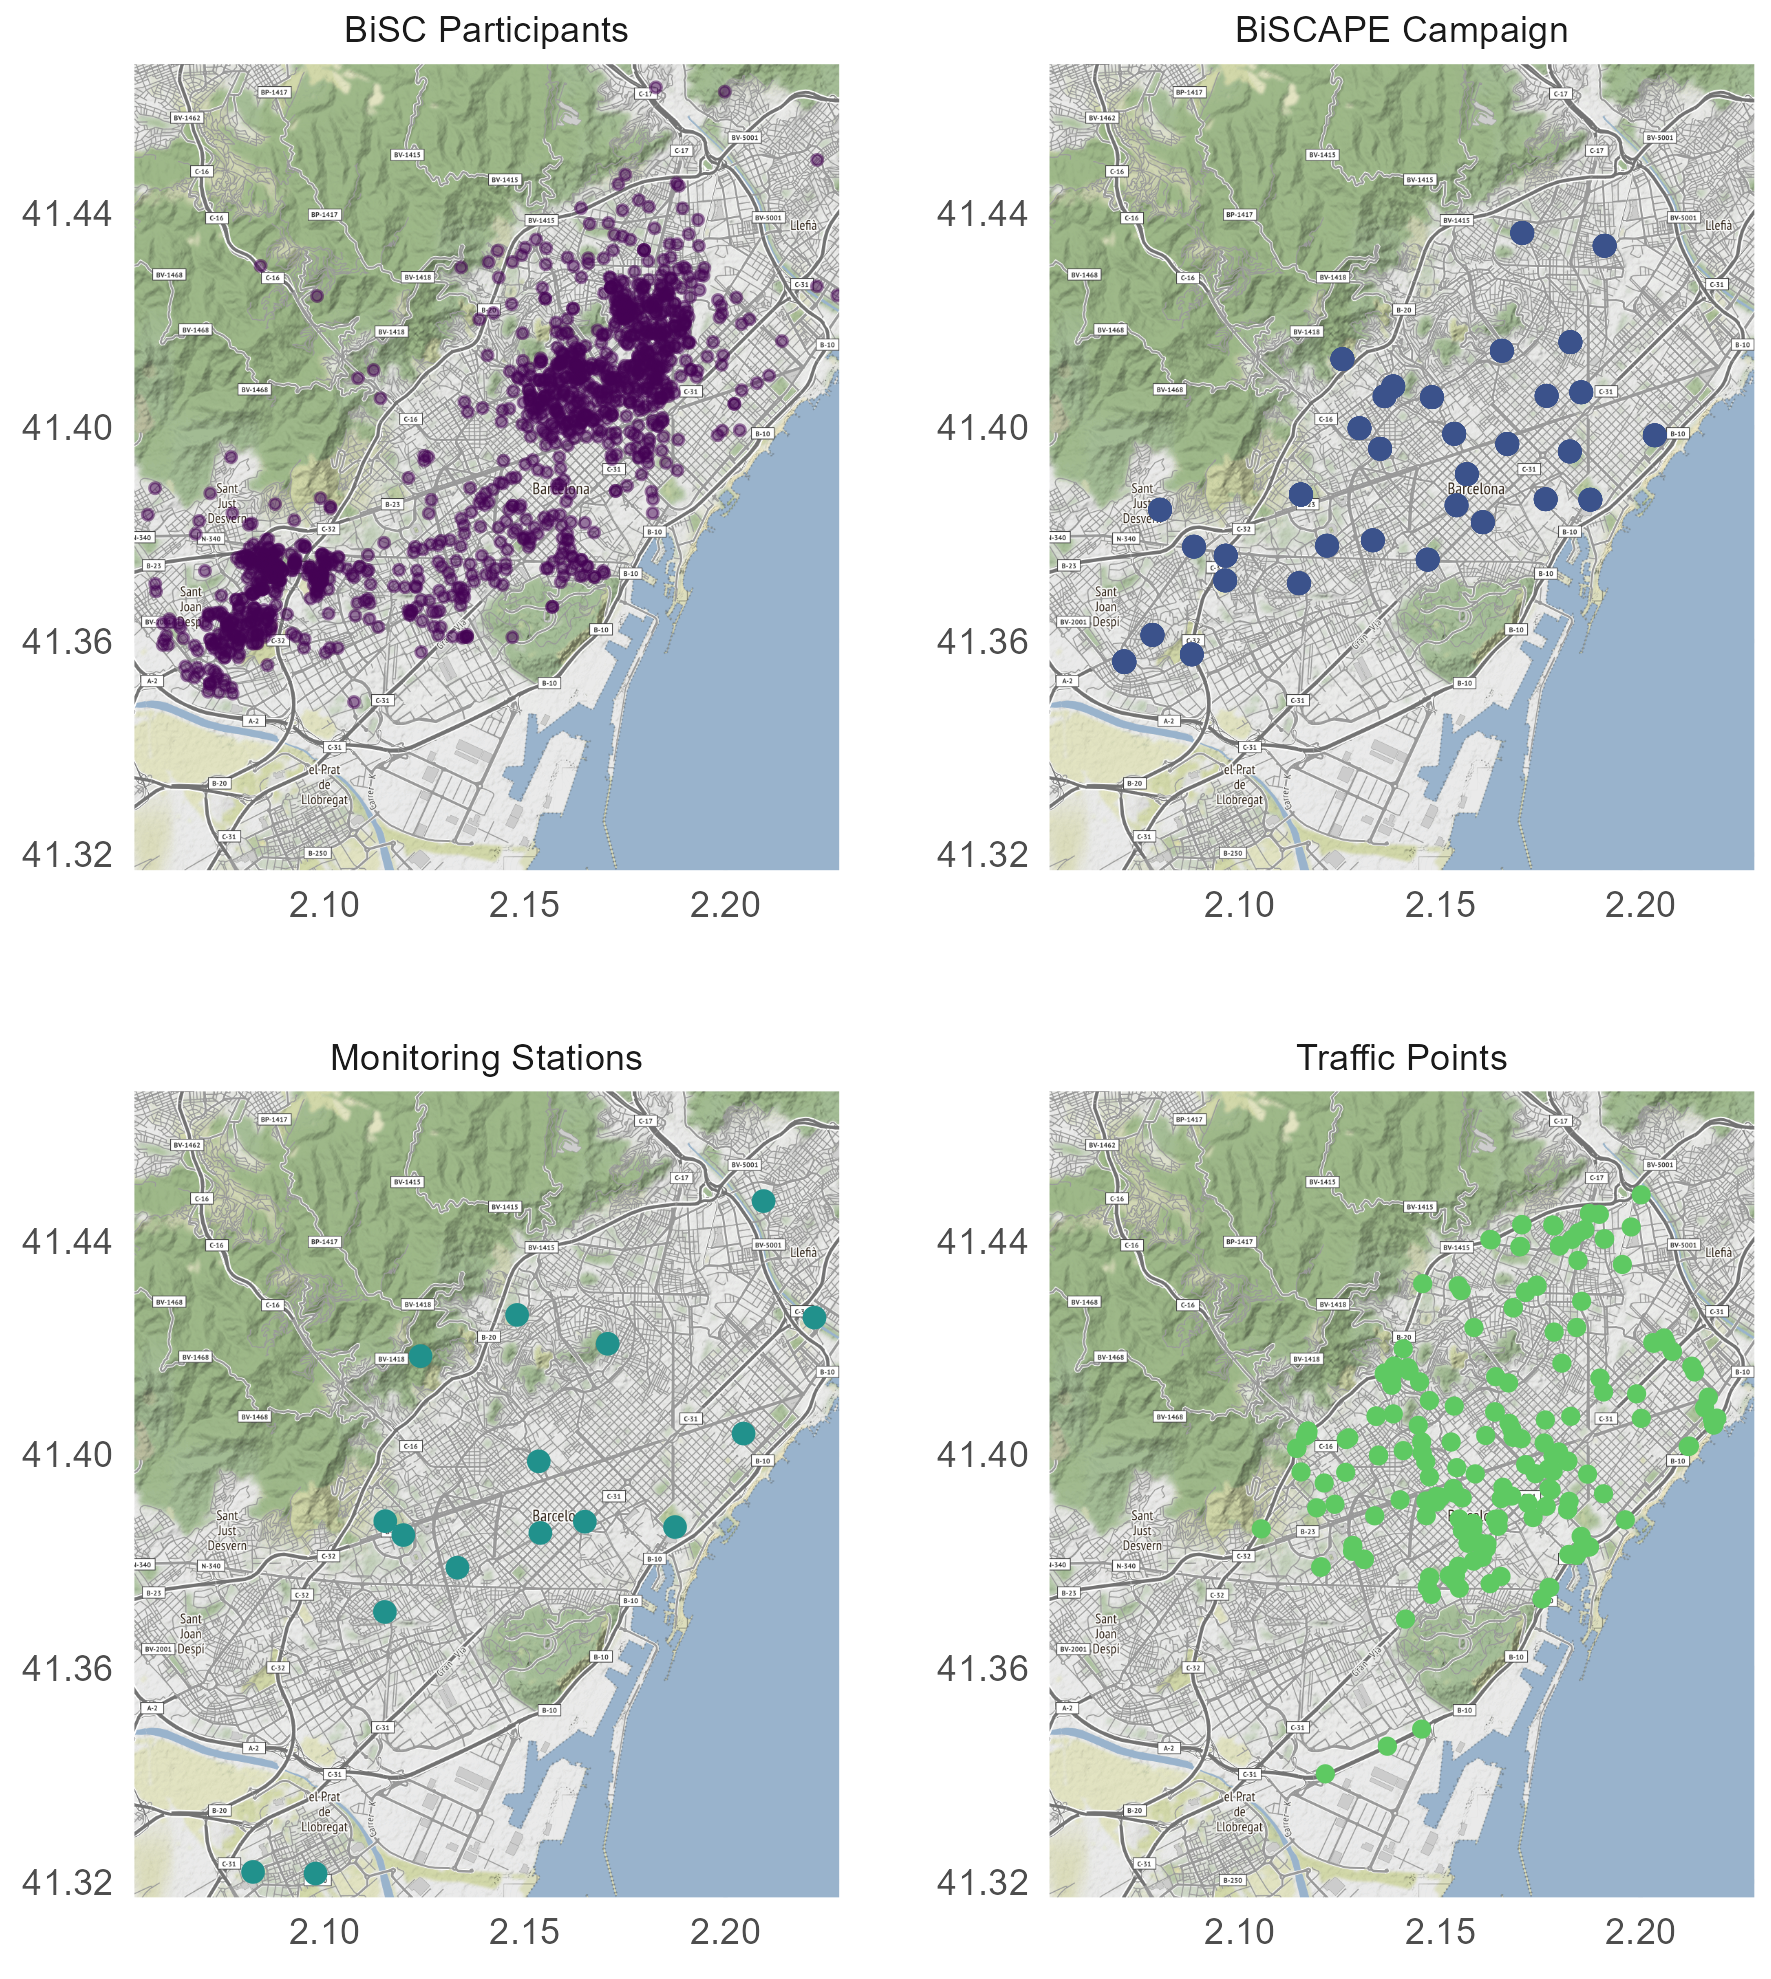
\includegraphics[width=1.0\textwidth]{figures/fig1_op2.png}
\caption{Study domain and spatial distribution (BiSC participants, BiSCAPE campaign, monitoring stations, and traffic points)}
\label{fig1}
\end{figure}

Air pollution measurements were conducted during two separate monitoring campaigns. The first, named the "BiSC-home" campaign, took place at the home addresses of BiSC participants and involved measuring only NO\textsubscript{2} levels for one week during the first, and third trimester of pregnancy between 2018-2021. The second campaign was carried out in accordance with the ESCAPE guidelines, named "BiSCAPE", and included four distinct measurement periods: three in the winter, summer, and autumn of 2021, and a final one in the winter of 2022. During these periods, levels of NO\textsubscript{2}, PM\textsubscript{2.5}, and BC were measured at 34 locations across Barcelona Metropolitan Area (Barcelona, Esplugues de Llobregat, and L'Hospitalet).These monitoring campaigns were used in the development of the LUR and HM.

%%%%%%%%%%%%%%%%%%%%%%%%%%
%%% --- LUR model --- %%%
%%%%%%%%%%%%%%%%%%%%%%%%%%
\subsection{LUR models}

LUR models for NO\textsubscript{2}  were developed using only data from the locations that had measured home-outdoor (BiSC-home campaign) levels for both sampling campaigns (i.e., we did not use data from participants who had data available for only one campaign, either first or third trimester). Almost half of the sites were measured before the COVID-19 pandemic started and half of the sites were during the pandemic period and its resulting restrictions. For PM\textsubscript{2.5}, PM\textsubscript{2.5} constituents, and BC models were developed using BiSCAPE data from the 34 sites.

For the development of the LUR models, spatial variables that better represent the pollutant concentration distribution across the study area were created. Following the ESCAPE guidelines \cite{eeftens2012, beelen2013},  predictor variables were selected from three broad categories: traffic, land use, and urban configuration. A wide variety of buffer sizes were created, i.e, 25m, 50m, 100m, 300m, 500m, and 1000m to capture the area-specific predictor variable at every single location.

We applied a supervised stepwise process in which we sequentially added a predictor variable to a linear regression model using pollutant concentrations as the independent variable to obtain the best possible model. This procedure was followed to build all the specific pollutant models. Previously to model development, we specified the direction expected of the effect that each predictor has in the model. For all predictor variables, univariate regression models with annual average air pollution concentration (NO\textsubscript{2}, PM\textsubscript{2.5}, PM\textsubscript{2.5} constituents (Fe, Zn, Cu, Sb), and BC) were conducted, models with the highest adjusted explained variance (R\textsuperscript{2}) were selected. We then repeated the process using the previous model and all the remaining predictor variables. Details of the LUR modelling and variables used can be found in the \textbf{Supplementary material X}.

%%%%%%%%%%%%%%%%%%%%%%%%%%%%%%%%%
%%% --- Dispersion model --- %%%
%%%%%%%%%%%%%%%%%%%%%%%%%%%%%%%%
\subsection{Dispersion models}

An emission inventory was compiled for the period 2018-2021, which included data from diverse emission sources such as vehicular traffic, household activities, industrial plants, airports, harbors, factories, and the commercial sector. The Atmospheric Dispersion Modelling System software (ADMS-Urban) from Cambridge Environmental Research Consultants (CERC) was employed to calculate the concentration of pollutants like NO\textsubscript{2}, PM\textsubscript{2.5}, PM\textsubscript{2.5} constituents (Fe, Zn, Cu, Sb), and BC originating from these sources. ADMS-Urban is a specialized Gaussian model designed for analyzing pollutant emissions in urban and metropolitan areas, particularly at road level \cite{mchugh1997adms}.

ADMS-Urban employs various algorithms to assess the chemical transportation and dispersion of pollutants, factoring in ground-level turbulence and turbulence induced by surrounding buildings \cite{stocker2012adms}. The model also features a meteorological pre-processing system that calculates fluxes and turbulence, enabling it to model airflow over complex terrains.

For enhanced accuracy, the dispersion model integrates data from a three-dimensional building and street width model from the Institut Cartogràfic i Geològic de Catalunya \cite{stoter2016state, 3Dcity}. This data aids in the calculation of the street canyon effect, a phenomenon characterized by tall buildings situated adjacent to heavily trafficked roads, which hinders atmospheric dispersion, leading to higher and relatively consistent pollutant concentrations compared to areas unaffected by the canyon effect.

The model also utilized meteorological data including wind speed, direction, air temperature, cloud cover, solar radiation, relative humidity, precipitation rate, and Planetary Boundary Layer Height (PBLH). This meteorological data was collected from the Zona Universitària station in Barcelona, managed by the Servei Meteorològic de Catalunya \cite{xema2013}.

To incorporate background pollution levels at a regional scale, data from Copernicus Atmosphere Monitoring Service Information (CAMS) was used. Background air pollution data has been extracted from the CAMS reanalysis ensemble model for 2018, and from CAMS ensemble forecast model for 2019-2020 \cite{cams2020, franceinstitut}. 

In addition, bias-adjustment techniques have been used to fit the model data to the observations. Through hourly bias spatial interpolation and generation of hourly maps. After that, data were processed  by cluster analysis techniques to obtain a mean cluster map. Each bias map by pollutant was associated to a cluster map class and an hourly-varying profile. 

Further details regarding the ADMS-Urban model and the variables used can be found in \textbf{Supplementary materials X}.

%%%%%%%%%%%%%%%%%%%%%%%%%%%%%
%%% --- Hybrid model --- %%%
%%%%%%%%%%%%%%%%%%%%%%%%%%%%
\subsection{Hybrid models}

For the hybrid models, we sought to improve their predictive power by integrating comprehensive data from multiple information sources and leveraging ML. For NO\textsubscript{2}, PM\textsubscript{2.5}, PM\textsubscript{2.5} constituents, and BC were largely based on daily concentrations from dispersion models, summarized as weekly averages, and spatial predictor variables from the LUR models. 

For a more comprehensive approach, we integrated additional data from the Catalan Air Pollution Monitoring and Forecasting Network (XVPCA) for Barcelona and surrounding areas \cite{xarxa2012}. This data was interpolated using the Inverse Distance Weighting (IDW) method, which assigns higher importance to nearest stations \cite{hoek2017methods}. The data came from 16 monitoring stations, including Ciutadella, Eixample, Gracia, Hospitalet, Ies Goya, Jardins, Observatori Fabra, Palau Reial, Plaza Universitària, Poblenou, Sagnier, Sants, St. Adria, St. Coloma, Vall Hebron, Zona Universitária \cite{xarxa2012}.

While our dispersion model initially utilized meteorological and traffic data, the hybrid model broadened its scope by integrating daily traffic counts from 180 locations throughout the city \cite{trafficbcn}. This broader data helps us better understand the spatial and time-specific variations in urban air pollution \cite{pinto2020}. To further refine our insights into the influence of weather patterns on pollution, we sourced additional meteorological variables, such as wind speed and air temperature, from the Raval monitoring station managed by Servei Meteorològic de Catalunya \cite{xema2013}.

We employed the RF algorithm to capture non-linear relationships and potential interactions between predictor variables and the response variable, utilizing \textit{the ranger package} in R implemented in the \textit{caret} framework \cite{wright2019}, a set of functions that attempt to streamline the process for creating predictive models \cite{caret2008}. Briefly, RF is a machine learning (ML) algorithm that constructs an ensemble of multiple decision trees \cite{breiman2001}. In this approach, each tree is formulated using a bootstrap sample of the data. During this process, every node within a tree represents the optimal split from a randomly selected subset of predictors. Predictions are then derived by averaging the outputs from all trees.

In summary, by combining data from multiple sources, our hybrid models aim to provide more accurate and reliable predictions. These predictions are essential for studying and mitigating urban air pollution. The distribution of the air pollution monitoring stations, meteorological stations, and traffic count measures are shown in the (\textbf{\cref{fig1}}, \textbf{Panel D}). 

%%%%%%%%%%%%%%%%%%%%%%%%%%%%%%%%%%%%%%%%%%%%%%%
%%% --- Model Evaluation and Comparison--- %%%
%%%%%%%%%%%%%%%%%%%%%%%%%%%%%%%%%%%%%%%%%%%%%%
\subsection{Performance assessment}

We evaluated model performance using various statistical approaches and on different temporal bases. The LUR models were evaluated on an annual basis, dispersion models were assessed both hourly and daily, and the hybrid models were evaluated on a weekly basis.

\subsubsection{LUR model evaluation}
Performance of the LUR models was assessed using \textit{k-fold cross-validation}. Specifically, we employed a 10-fold cross-validation technique. In this approach, the data was split into ten distinct sub-samples. For each iteration, the model was trained on k-1 folds and then validated using the leftover fold \cite{ziegel2003}. For every fold, we computed metrics such as \(R^2\), the root-mean-square-error (RMSE), mean bias (MB), and the correlation coefficient (\(r\)). After each iteration, both the error and adjusted \(R\textsuperscript{2}\) were recorded. This process was repeated \(k-times\), and the average of these measures was reported as the indicator of the model validity. 
\vspace{0.5cm} Details from the metrics used for model validation can be found in the \textbf{Supplementary material X}.

We carried out both internal and external validation for the NO\textsubscript{2} LUR model. Internal validation was conducted by applying a K-fold cross-validation analysis. The 10-fold cross-validation procedure and its significance have been detailed above. For the external validation of the NO\textsubscript{2} LUR model, we applied data from BiSC-home participants' homes for those participants who had data available only for one measurement campaign, and therefore their data were not used for developing NO\textsubscript{2} LUR model. For LUR models BC, PM\textsubscript{2.5}, and its constituents (Cu, Fe, Sb, and Zn), internal validation was conducted using the \textit{leave-one-out-cross-validation (LOOCV)} process. For these models, we were not able to conduct external validation due to the lack of external data.

\subsection{Dispersion model evaluation}
Dispersion models were evaluated by comparing the yielded results from the ADM-Urban model with the real values measured by the air quality stations (XVPCA), including Ciutadella, Eixample, Gracia, Palau Reial, Poblenou, Sants, among others. Details from the metrics used for dispersion model validation can be found in the \textbf{Supplementary material X}.\vspace{0.5cm} 

\subsection{Hybrid model evaluation}
We assessed the performance of each hybrid model by contrasting predictions with observations. Two distinct validation approaches were employed: the \textit{10-fold cross-validation} and the \textit{out-of-bag (OBB) score}. While both methods vary in the sample size designated for training and testing, their core difference lies in the data-splitting strategy. In the 10-fold CV, the model trains on nine out of the ten data partitions and then validates against the remaining one. In contrast, the OOB approach trains the model on two-thirds of the data and uses the residual third for external validation. We follow a grid search for hyperparameter tuning  to select the best configuration to obtain the optimal model based on the \textit{Root Mean Squared Error (R\textsuperscript{2})}. 

All statistical analyses were performed in R version 4.3.1 \cite{Rstudio}. GIS predictor variables were computed using X software. 

\newpage
%%%%%%%%%%%%%%%%%%%%%%%%
%%% --- Results --- %%%
%%%%%%%%%%%%%%%%%%%%%%%
\section{Results}

%%%%%%%%%%%%%%%%%%%%%%%%%%%%%%%%%%%%%%%%%%%%%%%%%%%%%
% --- Distribution of the monitoring campaigns --- % 
%%%%%%%%%%%%%%%%%%%%%%%%%%%%%%%%%%%%%%%%%%%%%%%%%%%%

\subsection{Distribution of monitoring campaigns}

Distribution of the observed concentration for the BiSC-home and BiSCAPE campaigns for all pollutants are shown in \hyperref[table1]{Table 1}. NO\textsubscript{2} concentration levels for the combination of BiSC-home and BiSCAPE campaigns ranged between 6.85 \(\mu \text{g/m}^3\) and 97.3 \(\mu \text{g/m}^3\) with a mean (sd) of  38.8 (12.4) \( \mu \text{g/m}^3\). PM\textsubscript{2.5} observed levels ranged between 6.14 \(\mu \text{g/m}^3\) and 35.8 \( \mu \text{g/m}^3\) with a mean (sd) of 13.4 (6.14) \(\mu \text{g/m}^3\), while BC levels showed less variation during the BiSCAPE campaign ranged between 0.40 \(\mu \text{g/m}^3\) and 2.95 \(  \mu \text{g/m}^3\) with a mean of 1.27 (0.50) \( \mu \text{g/m}^3\). For PM\textsubscript{2.5} constituents concentration values observed during the BiSCAPE campaign varied substantially between elements with a mean of 0.25 for  FE,  7.10 for Cu, and a mean of 40.7 for Mn. 


\\
The spatial distribution of the outdoor air pollution measurements campaigns were showed in \cref{fig1}.  Panel Fig 1.A show a high density coverage  

%%% ---------------------------------------------------------------- %%%
%%% Table 1. Outdoor air pollution concentration BiSC-home, BiSCAPE  %%%
%%% ---------------------------------------------------------------  %%%
\begin{table}[h!]
\centering
\caption{Outdoor air pollution concentration distribution for the BiSC-home and BiSCAPE campaigns (2018-2022)}
\begin{tabular}{lllllllllll} % each one indicates a new column in the table 
\toprule
Campaign & Pollutant & Year  & mean & sd & min & p25 & p50 & p75 & max \\ 
\midrule
BiSC-home, BiSCAPE & NO\textsubscript{2} (\mu\)g/m\textsuperscript{3}) & 2018-2021 & 38.8 & 12.4 & 6.85 &30.0 & 37.5 & 45.8 & 97.3 \\ 
\multirow{5}{*}{BiSCAPE} 
& PM\textsubscript{25} (\(\mu\)g/m\textsuperscript{3}) & 2021-2022  & 13.4 & 6.14 & 5.01 & 9.06 & 11.3 & 16.2 & 35.8 \\ 
& BC (\(\mu\)g/m\textsuperscript{3}) & 2021-2022  & 1.27 & 0.50 & 0.40 & 0.88 & 1.22 & 1.52 & 2 .95 \\ 
& Fe (\(\mu\)g/m\textsuperscript{3}) & 2021-2022  & 0.25 & 0.13 & 0.07 & 0.15 & 0.21 & 0.32 & 0.77 \\ 
& Cu (ng/m\textsuperscript{3}) & 2021-2022 & 7.10 & 3.82 & 1.78 & 4.37 & 6.36 & 8.98 & 22.7 \\ 
& Mn (ng/m\textsuperscript{3}) & 2021-2022  & 40.7 & 36.5 & 6.71 &  18.9 & 28.2 & 46.7 & 273 \\ 
\bottomrule
\end{tabular}
\end{table}


Since different approaches were used to built outdoor air pollution models these were not directly comparable due to differences on temporal basis. 

The performance of the models varied substantially by pollutant. In table x. performance metrics for the HM are shown. Hybrid BC model had the best performance of the models assessed, with a higher R\textsuperscript{2} and lower RMSE. Performance metrics for LUR, DM and HM are shown in the supplementary materials. 


% --- Exposure concentrations --- %
Predictions from outdoor air pollution concentration exposure during the entire pregnancy for each pollutant and model is shown in FIGURE X. The exposure range was larger for the LUR model for all the pollutants assessed. Dispersion model predicted lower exposure concentration values than LUR and Hybrid. In addition to that HM show less variability in the exposure concentration.

%%% -------------------------------------------%%%%
%%% --- Figure 2. Boxplot models comparison --- %%%
%%% -------------------------------------------%%%%
\begin{figure}[!htb]
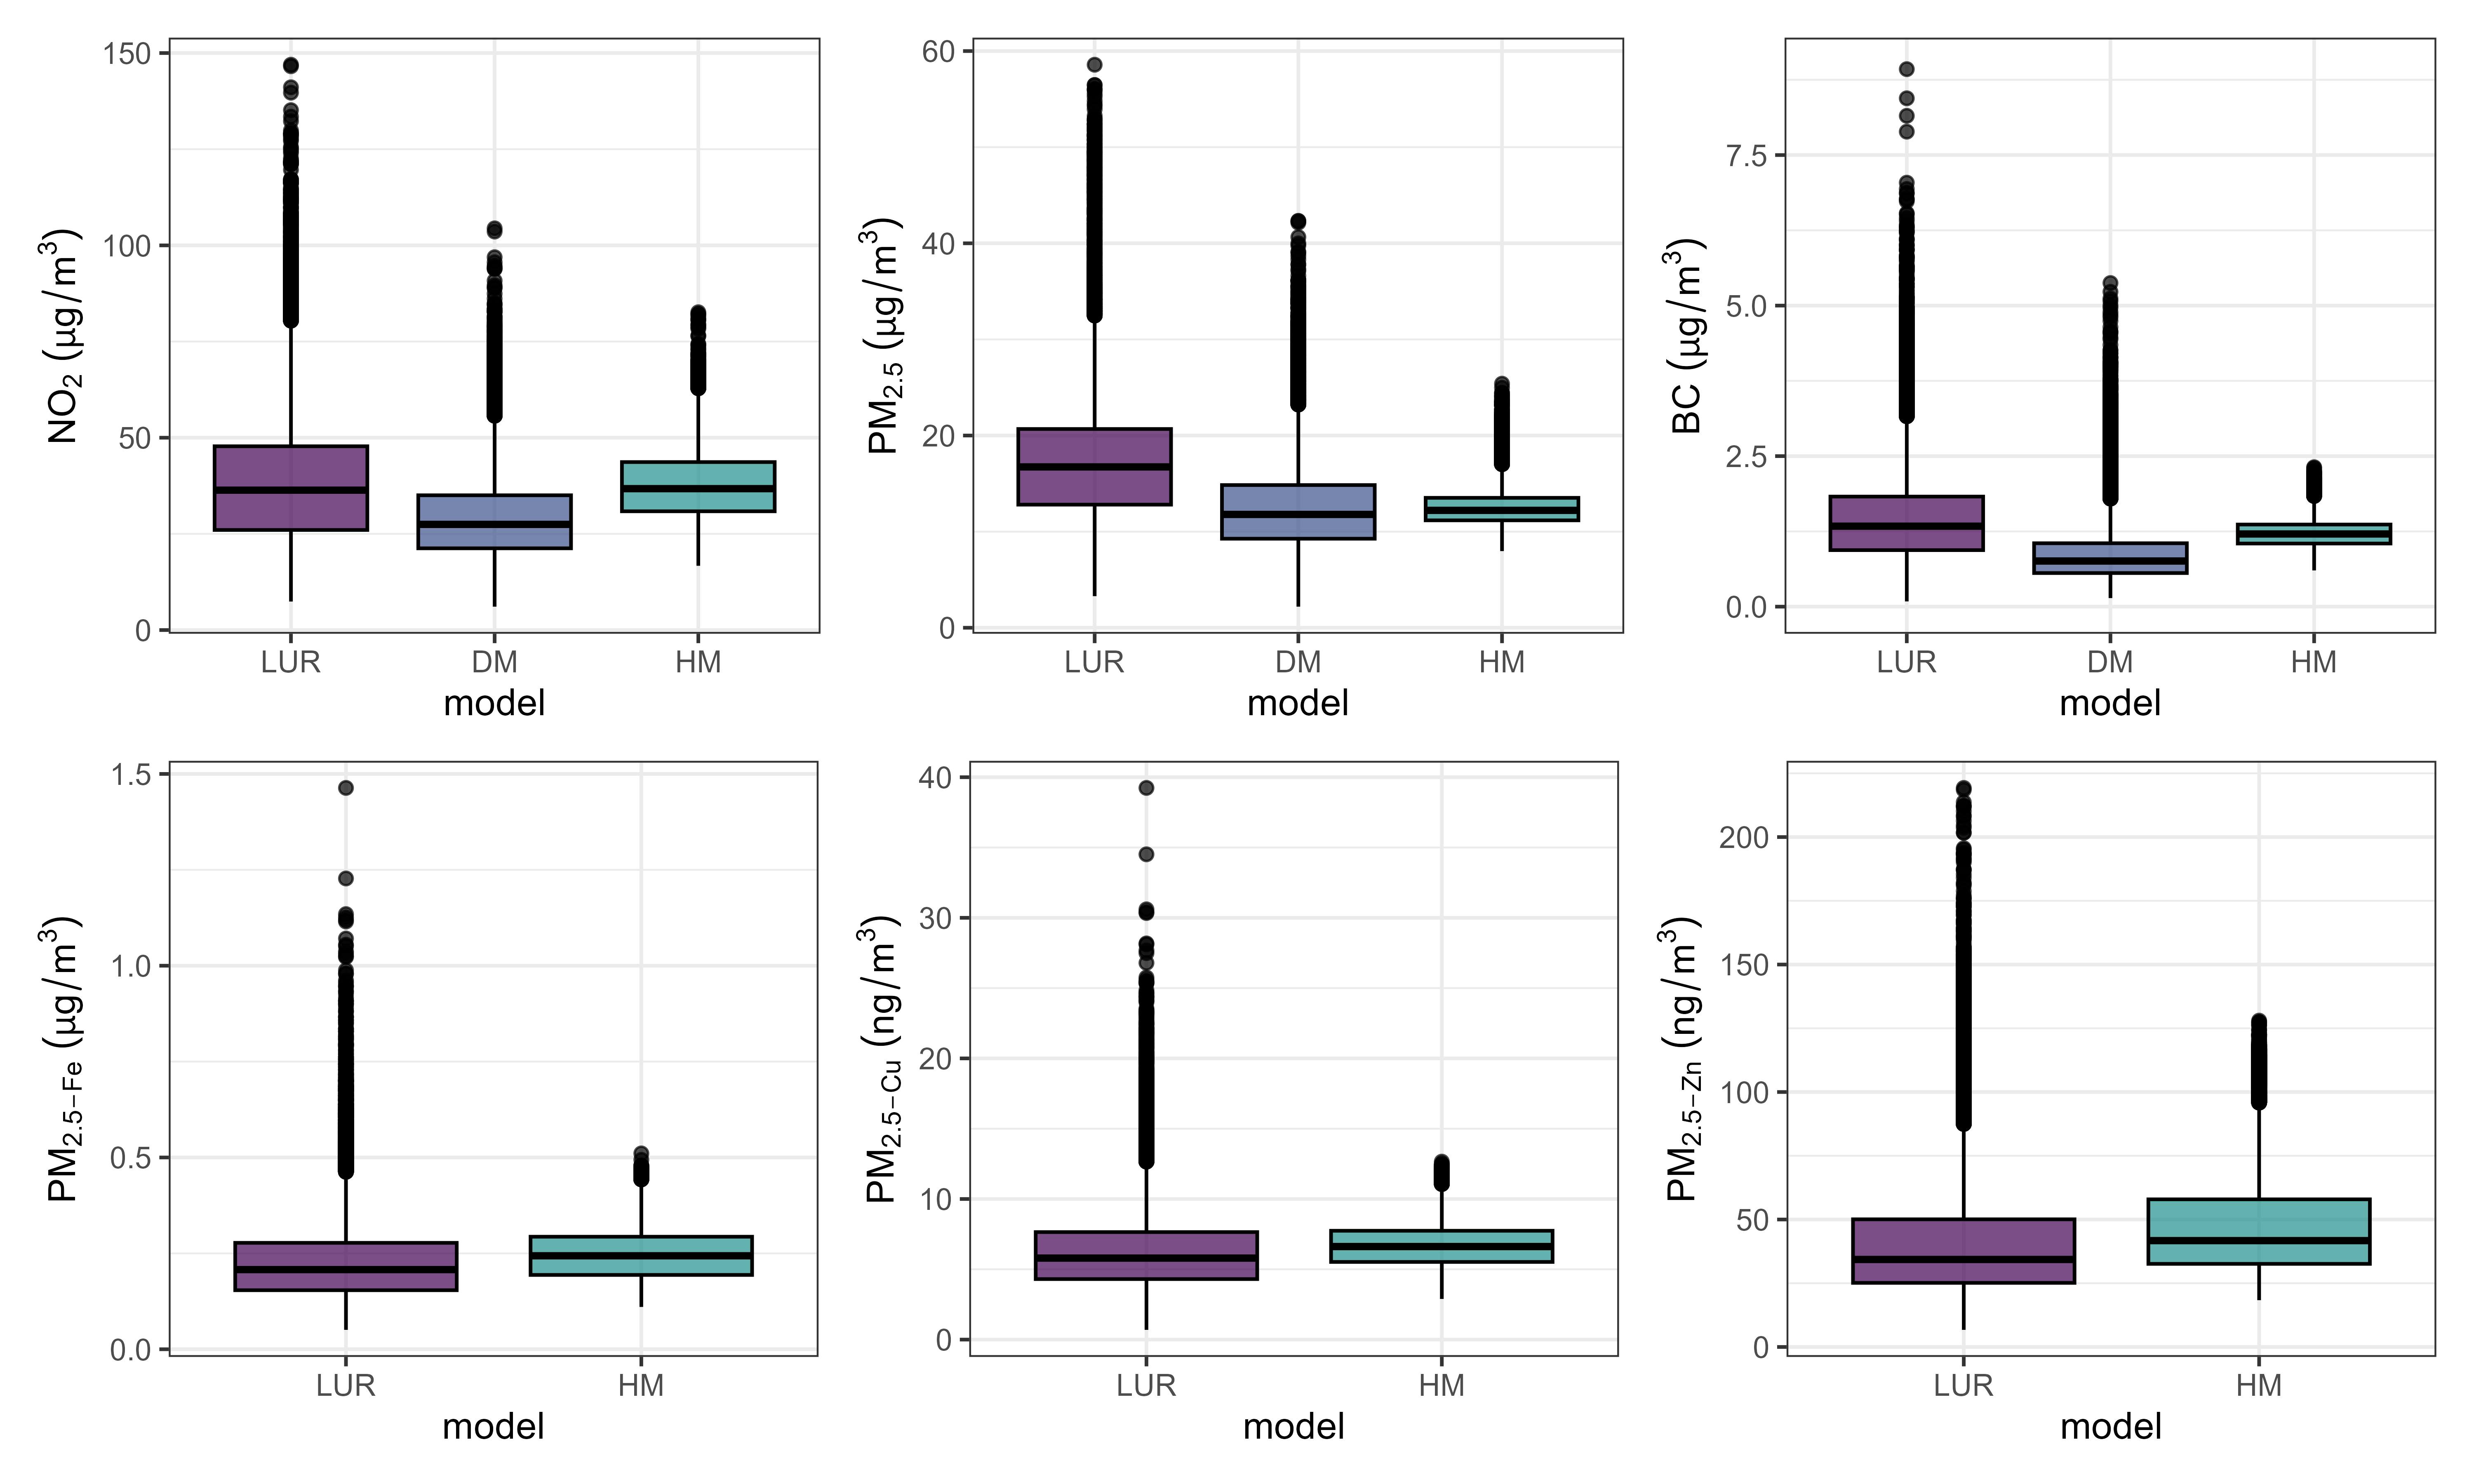
\includegraphics[width=1.0\textwidth]{figures/boxplot_all_models_estimates.png}
\caption{Distribution of exposure to air pollution during the entire pregnancy period for each exposure assessment model (\textit{NO$_2$}, \textit{PM$_{2.5}$}, \textit{BC}, \textit{Fe}, \textit{Cu}, \textit{Zn})}
\end{figure}


\textbf{\cref{fig2}} presents the distribution of the observed and estimated NO\textsubscript{2}, PM\textsubscript{2.5} and BC concentrations from the LUR, DM, and HM. The data shown are long-term estimated concentrations of pollutants, after averaging weekly estimates for all the study period (2019 - 2021).   


\newpage

%%%%%%%%%%%%%%%%%%%%%%%%%%%%%%%%%%%%%%%%%%%%%%%%%%%%%%%%%%%%%%%%%%%%%%%%%
%%% --- Spatial distribution of outdoor air pollution estimates  --- %%%
%%%%%%%%%%%%%%%%%%%%%%%%%%%%%%%%%%%%%%%%%%%%%%%%%%%%%%%%%%%%%%%%%%%%%%%%%

%%% --- Figure. Average exposure during the entire pregnancy period --- %%%
% Put the figure text closer to the Figure 3
\captionsetup[figure]{skip=6pt}
% We add the figure with the study domain 
\begin{figure}[!htb]
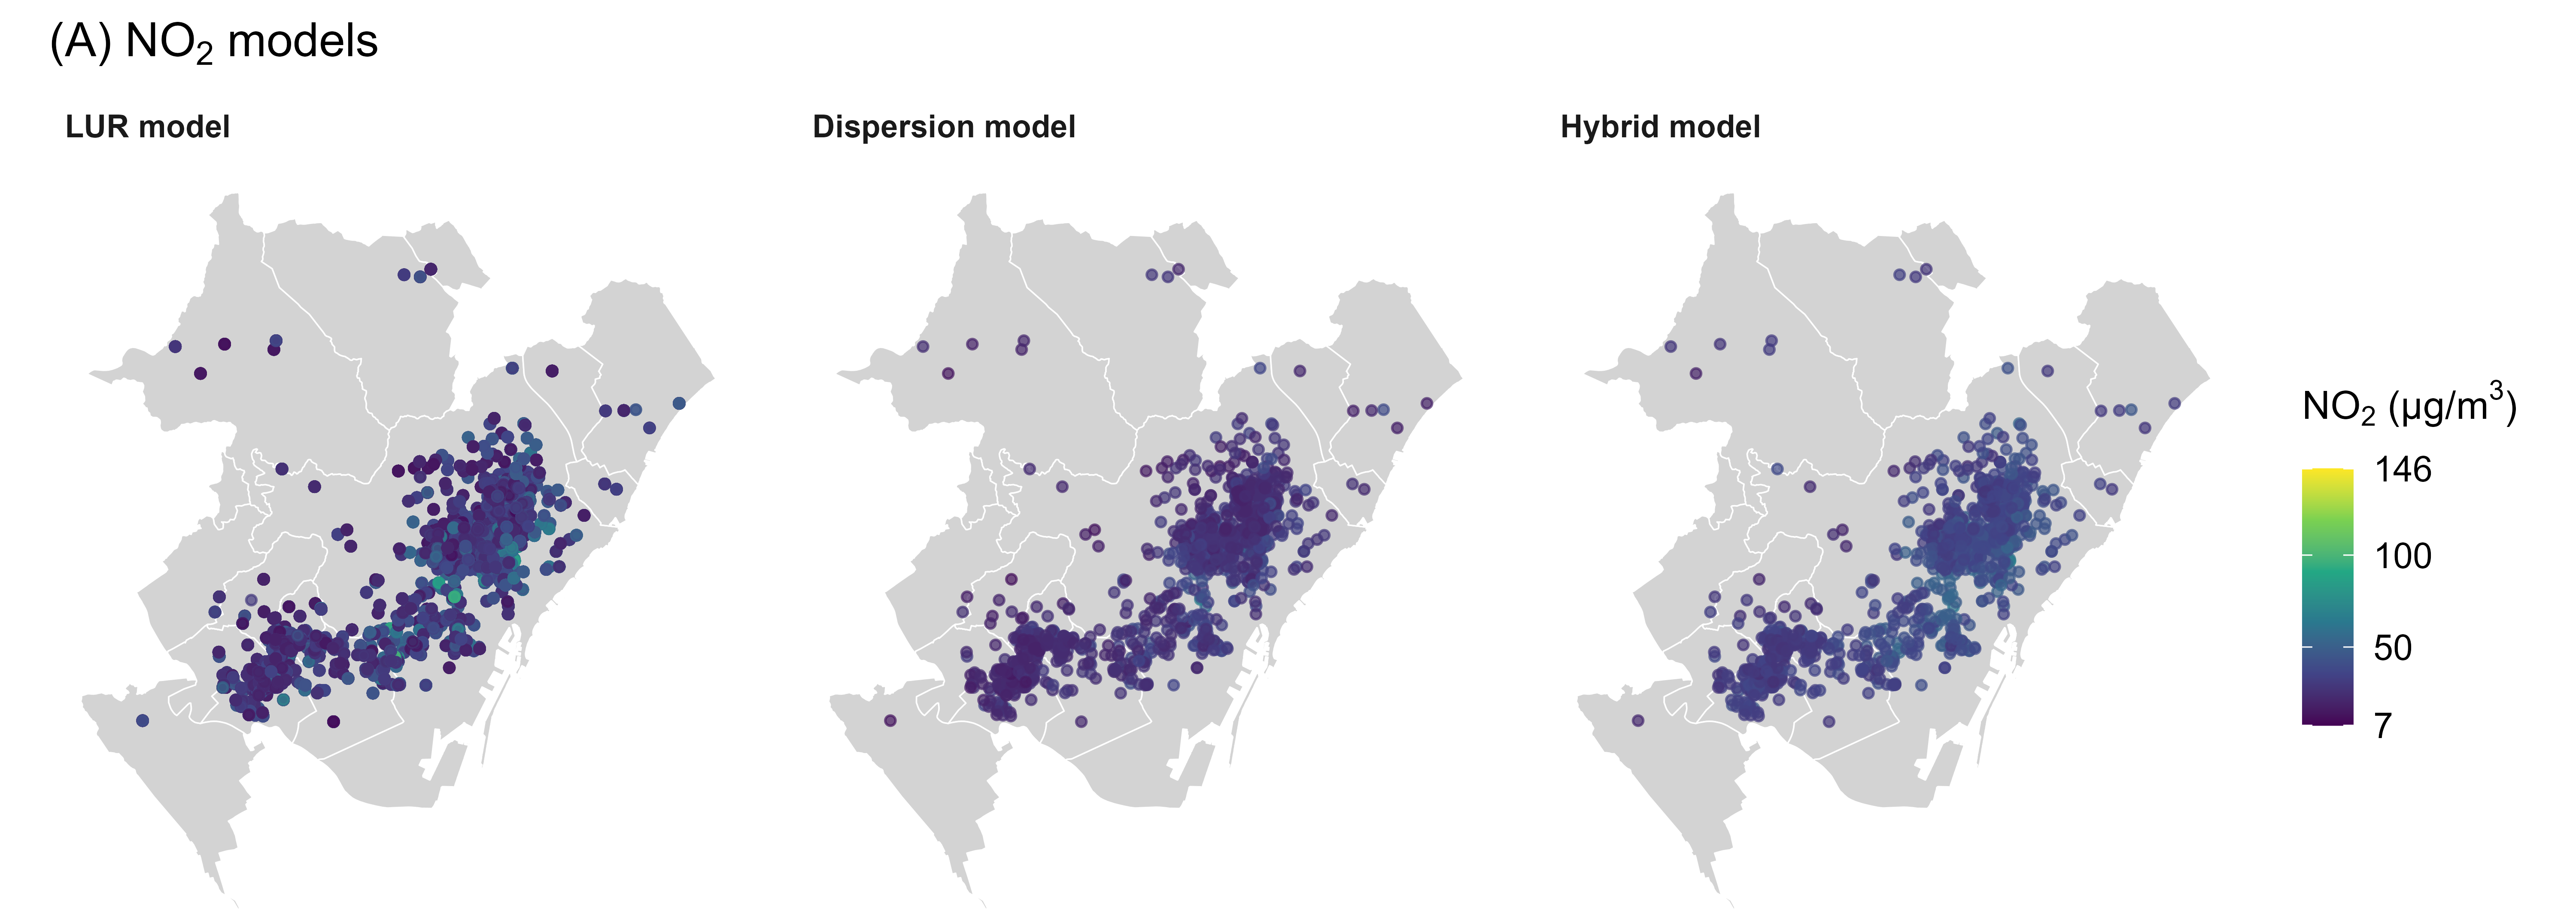
\includegraphics[width=1.0\textwidth]{figures/NO2_models_map.png}
\end{figure}

% Put the figure text closer to the Figure 3
\captionsetup[figure]{skip=6pt}
% We add the figure with the study domain 
\begin{figure}[!htb]
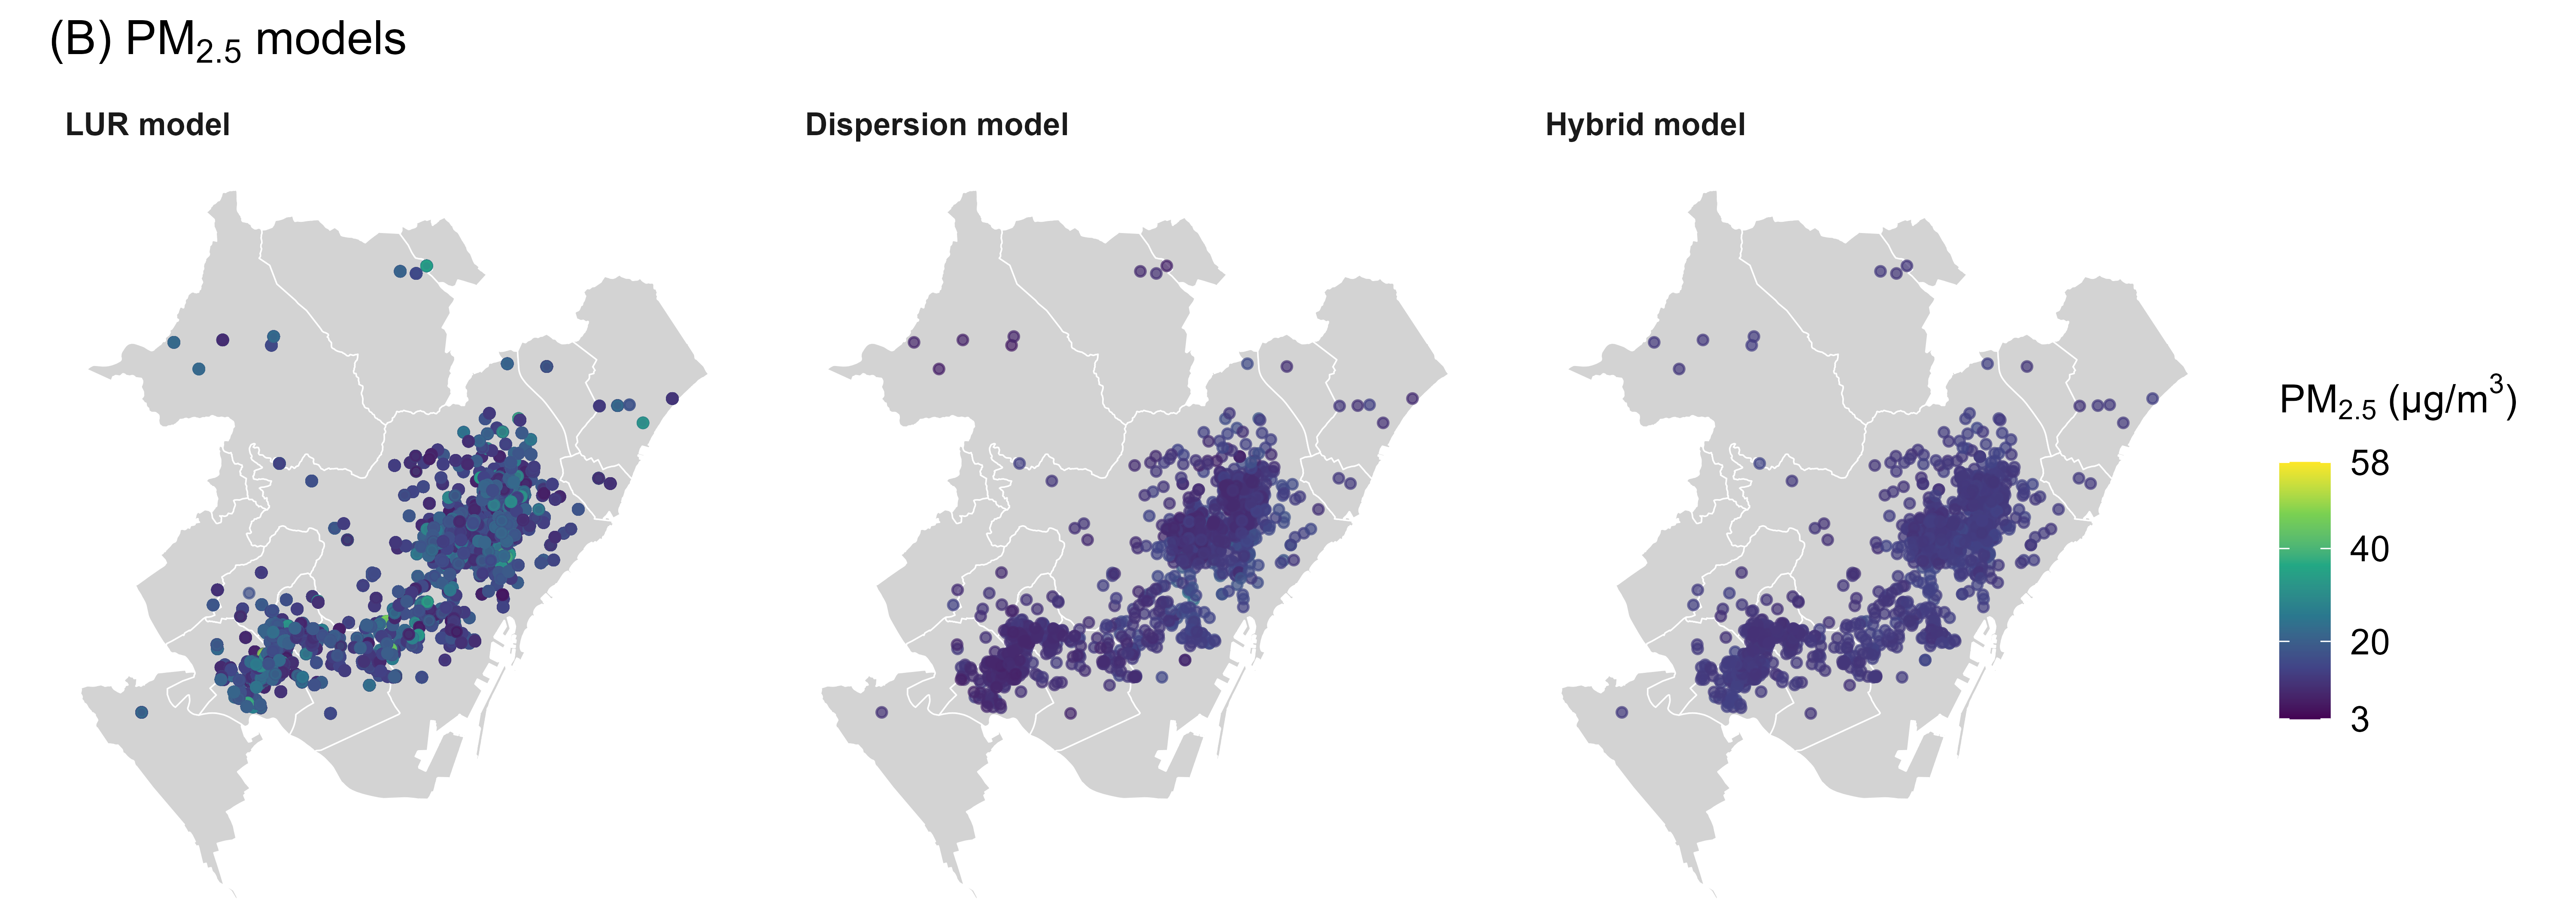
\includegraphics[width=1.0\textwidth]{figures/PM25_models_map.png}
\end{figure}

% Put the figure text closer to the Figure 3
\captionsetup[figure]{skip=6pt}
% We add the figure with the study domain 
\begin{figure}[!htb]
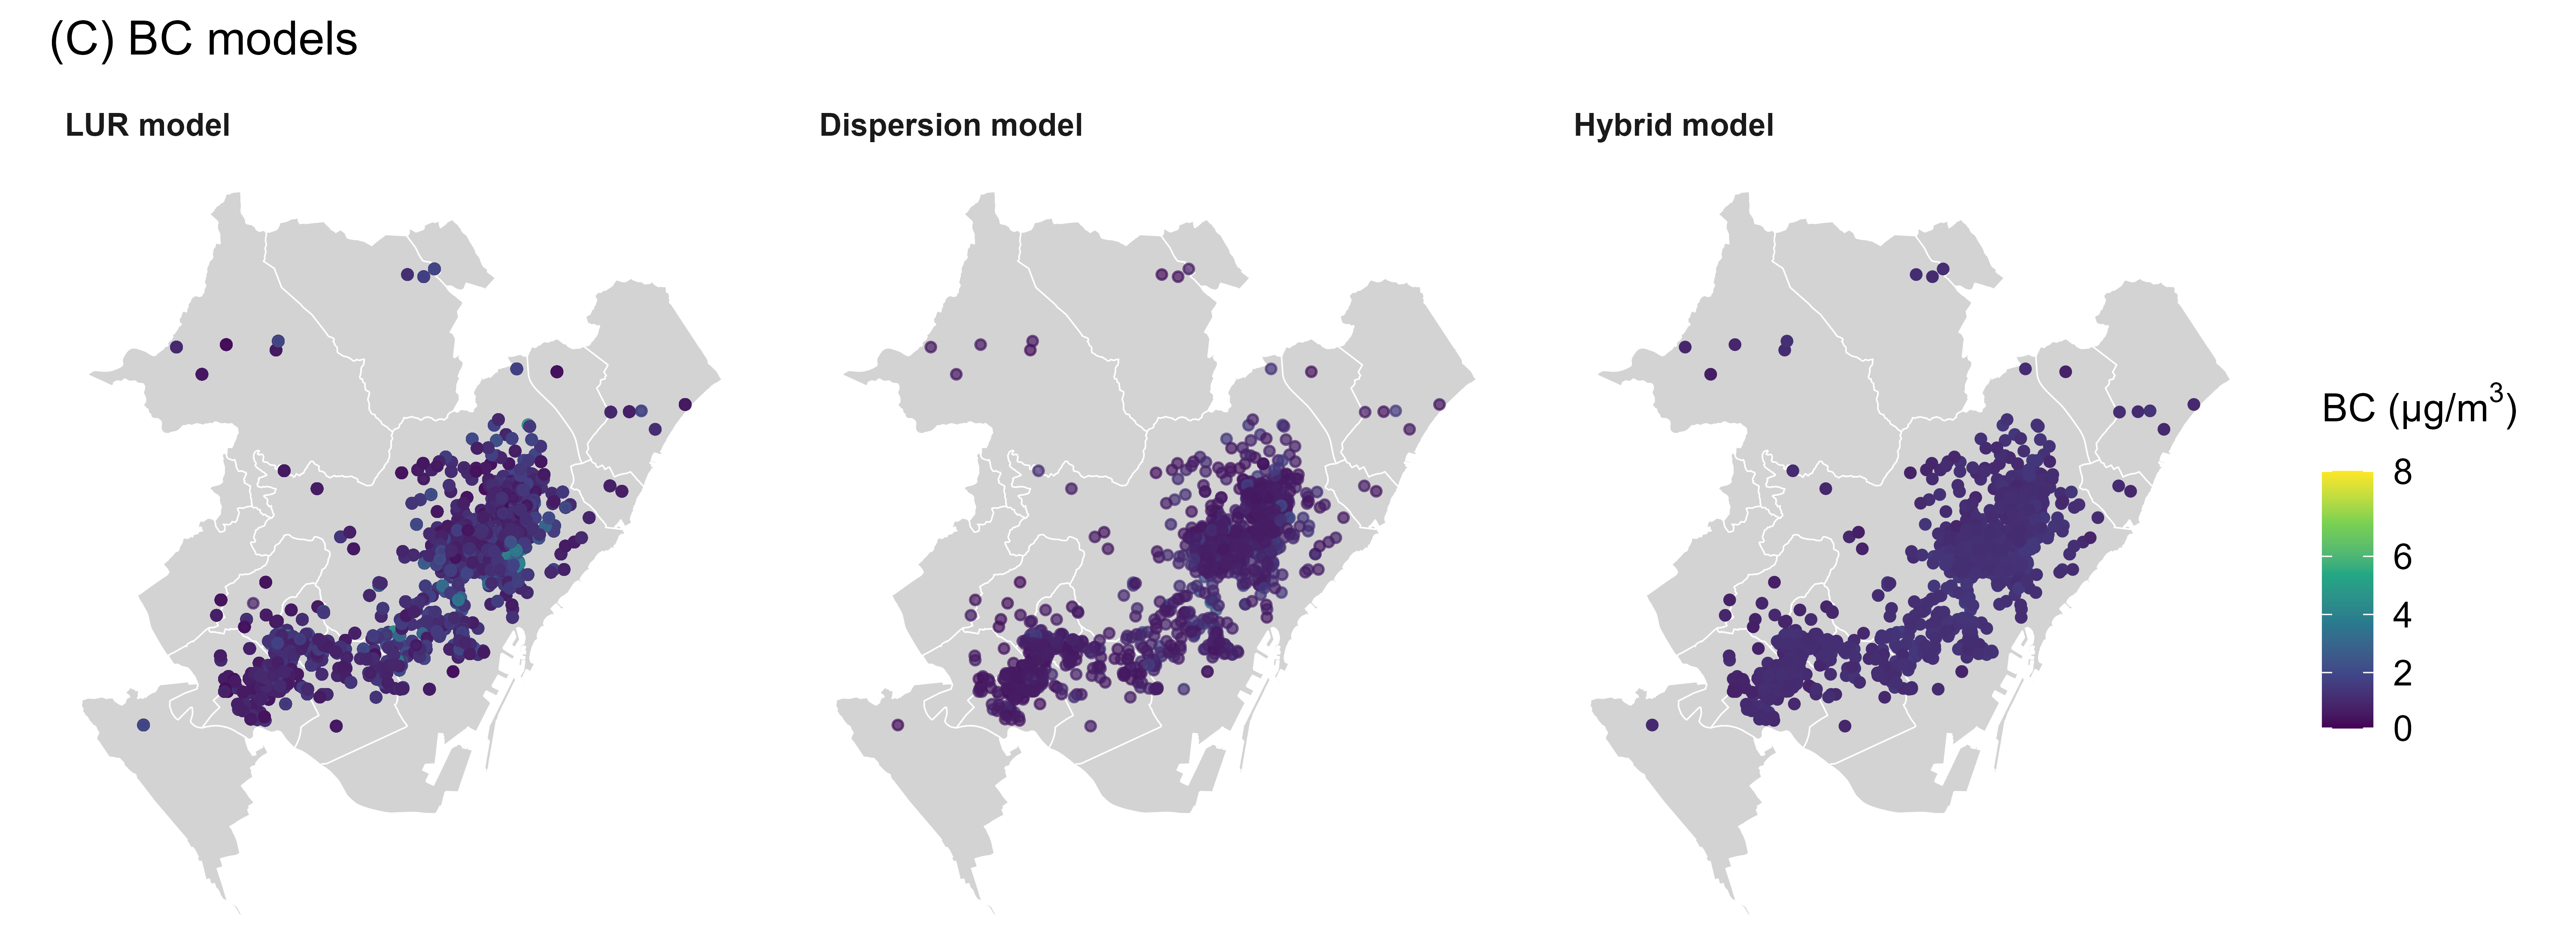
\includegraphics[width=1.0\textwidth]{figures/BC_models_map.png}
\caption{Pregnancy exposure for the entire pregnancy period \textit{NO$_2$}, \textit{PM$_{2.5}$}, \textit{BC}.}
\end{figure}


\newpage
%%%%%%%%%%%%%%%%%%%%%%%%%%%%%%%%%%%%%%%%%%%%%%%%%%%%%%%%%%%%%
% --- Correlation between measures and model estimates --- %
%%%%%%%%%%%%%%%%%%%%%%%%%%%%%%%%%%%%%%%%%%%%%%%%%%%%%%%%%%%%
Correlation for long-term exposure (entire pregnancy) at the residential addresses ranged from r = 0.48 to 0.92 \textbf{(figure 4.A)}. Correlation for short-term exposure (weekly exposure) varied from r = 0.37 to 0.90 \textbf{(figure 4.B)}. Correlation between the air pollutant estimates for the different models assessed was moderate to strongly correlated for both long-and-short term exposure. Nitrogen dioxide 

% Here add the correlation plot (long and short term)
\captionsetup[figure]{skip=6pt}
% We add the figure with the study domain 
\begin{figure}[!htb]
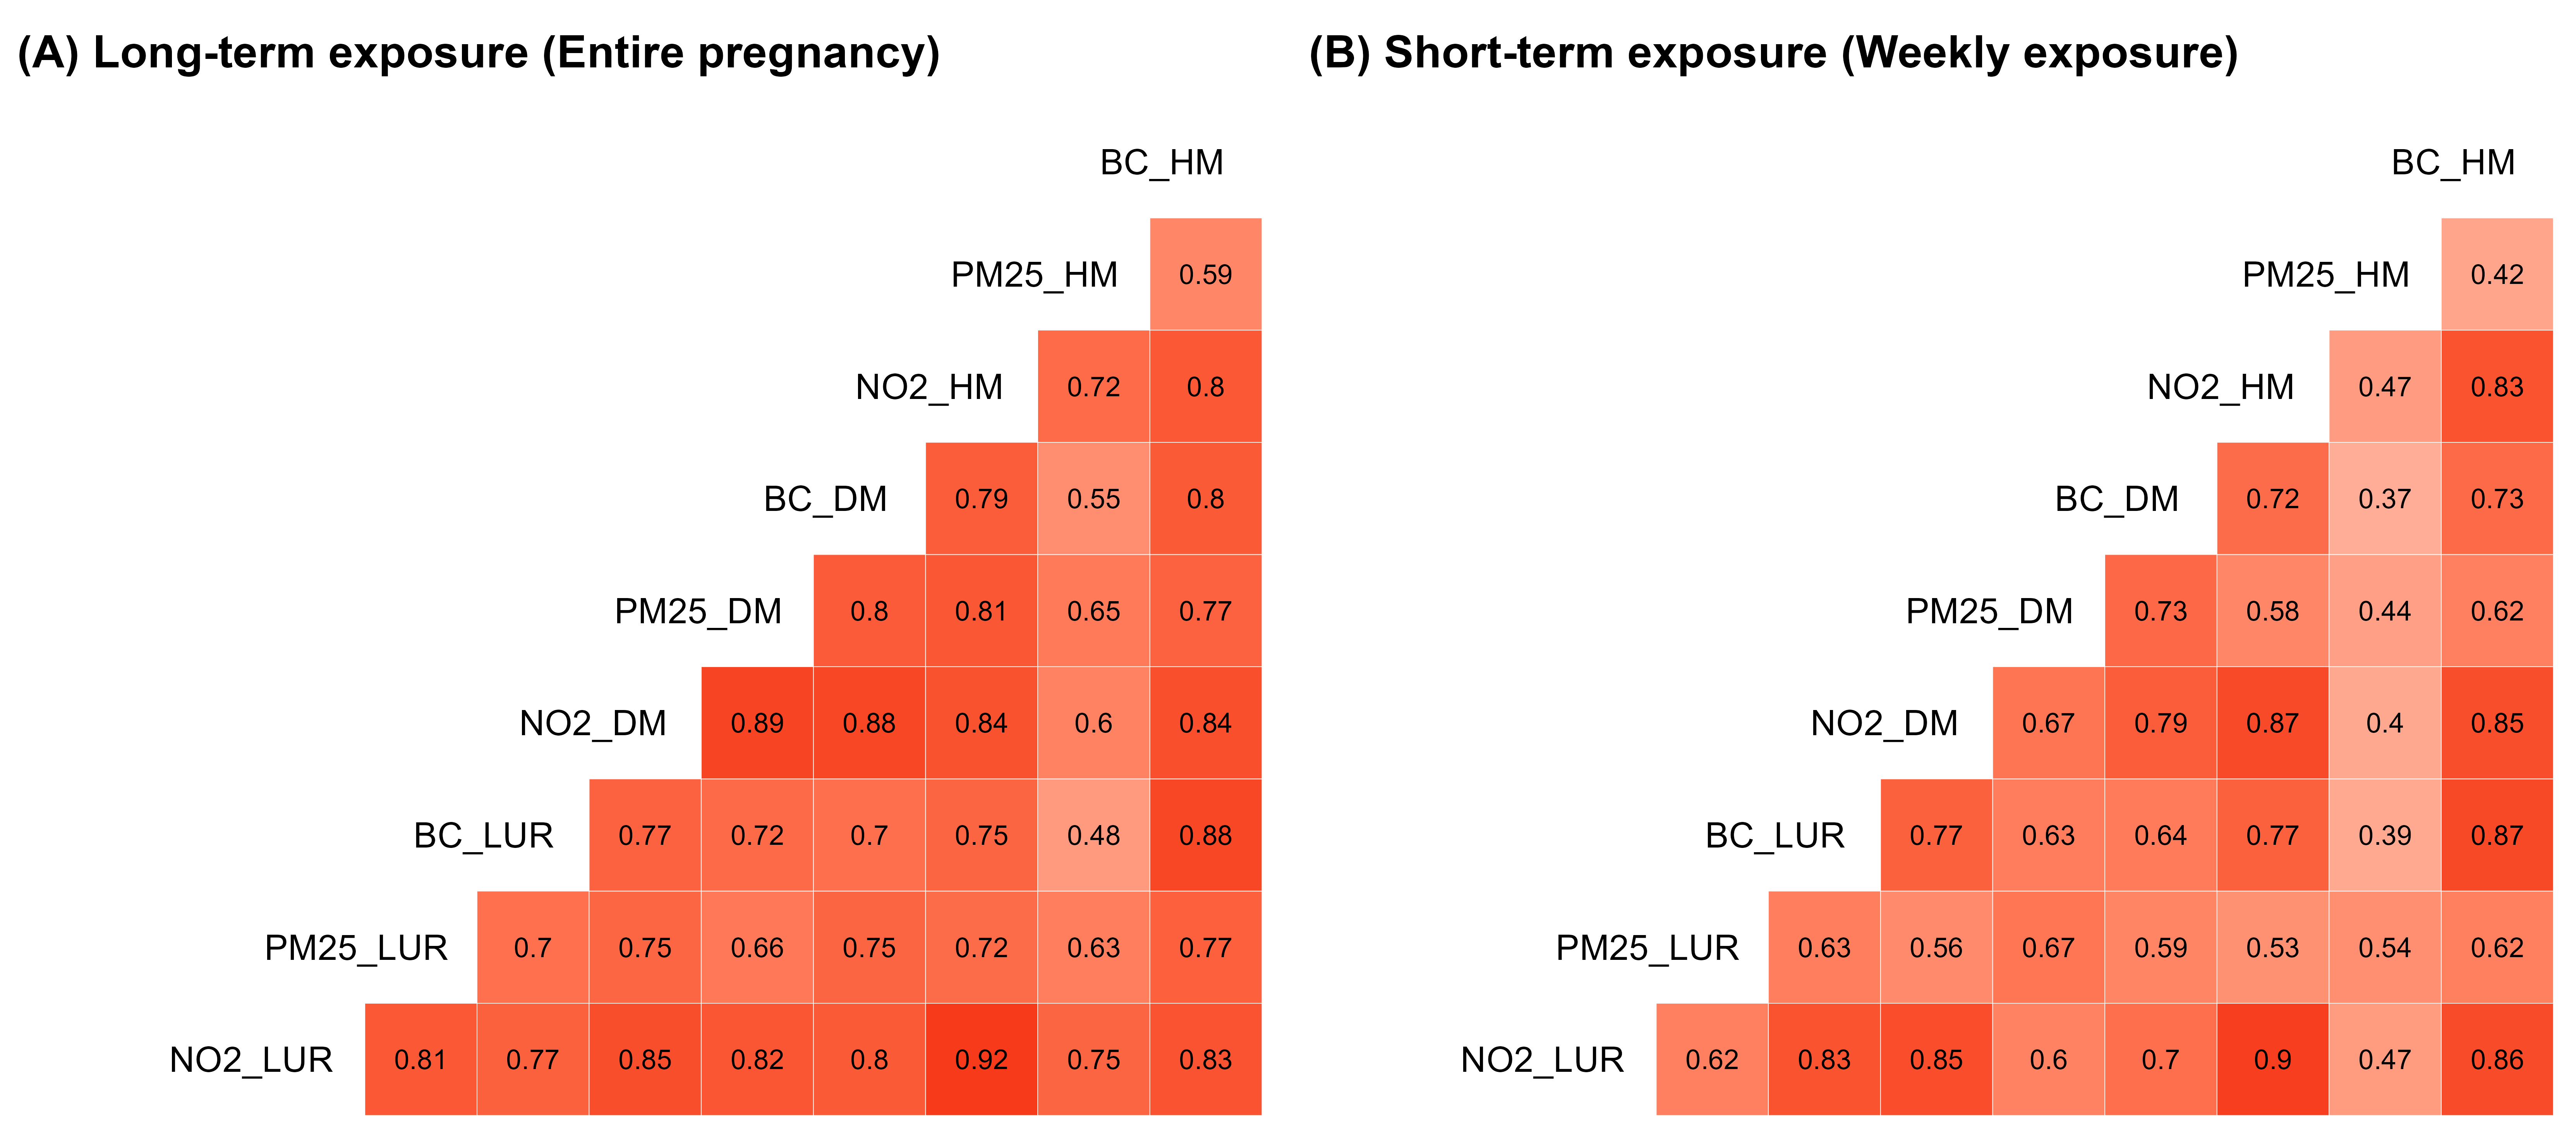
\includegraphics[width=1.0\textwidth]{figures/correlation_fig.png}
\caption{Correlation between traffic-related air pollutants for LUR, DM, HM in different windows of exposure \textit{NO$_2$}, \textit{PM$_{2.5}$}, \textit{BC}.}
\end{figure}



\newpage
%%%%%%%%%%%%%%%%%%%%%%%%%%%%%%%%%%%%%%%%%%%%%%%%%%%%%%%%%%%%%%%%%
% --- Comparison/agreement between air pollution estimates --- %
%%%%%%%%%%%%%%%%%%%%%%%%%%%%%%%%%%%%%%%%%%%%%%%%%%%%%%%%%%%%%%%%

%%% --- Figure. Comparison/agreement between moodel predictions estimates --- %%%
% Put the figure text closer to the Figure 3
\captionsetup[figure]{skip=6pt}
% We add the figure with the study domain 
\begin{figure}[!htb]
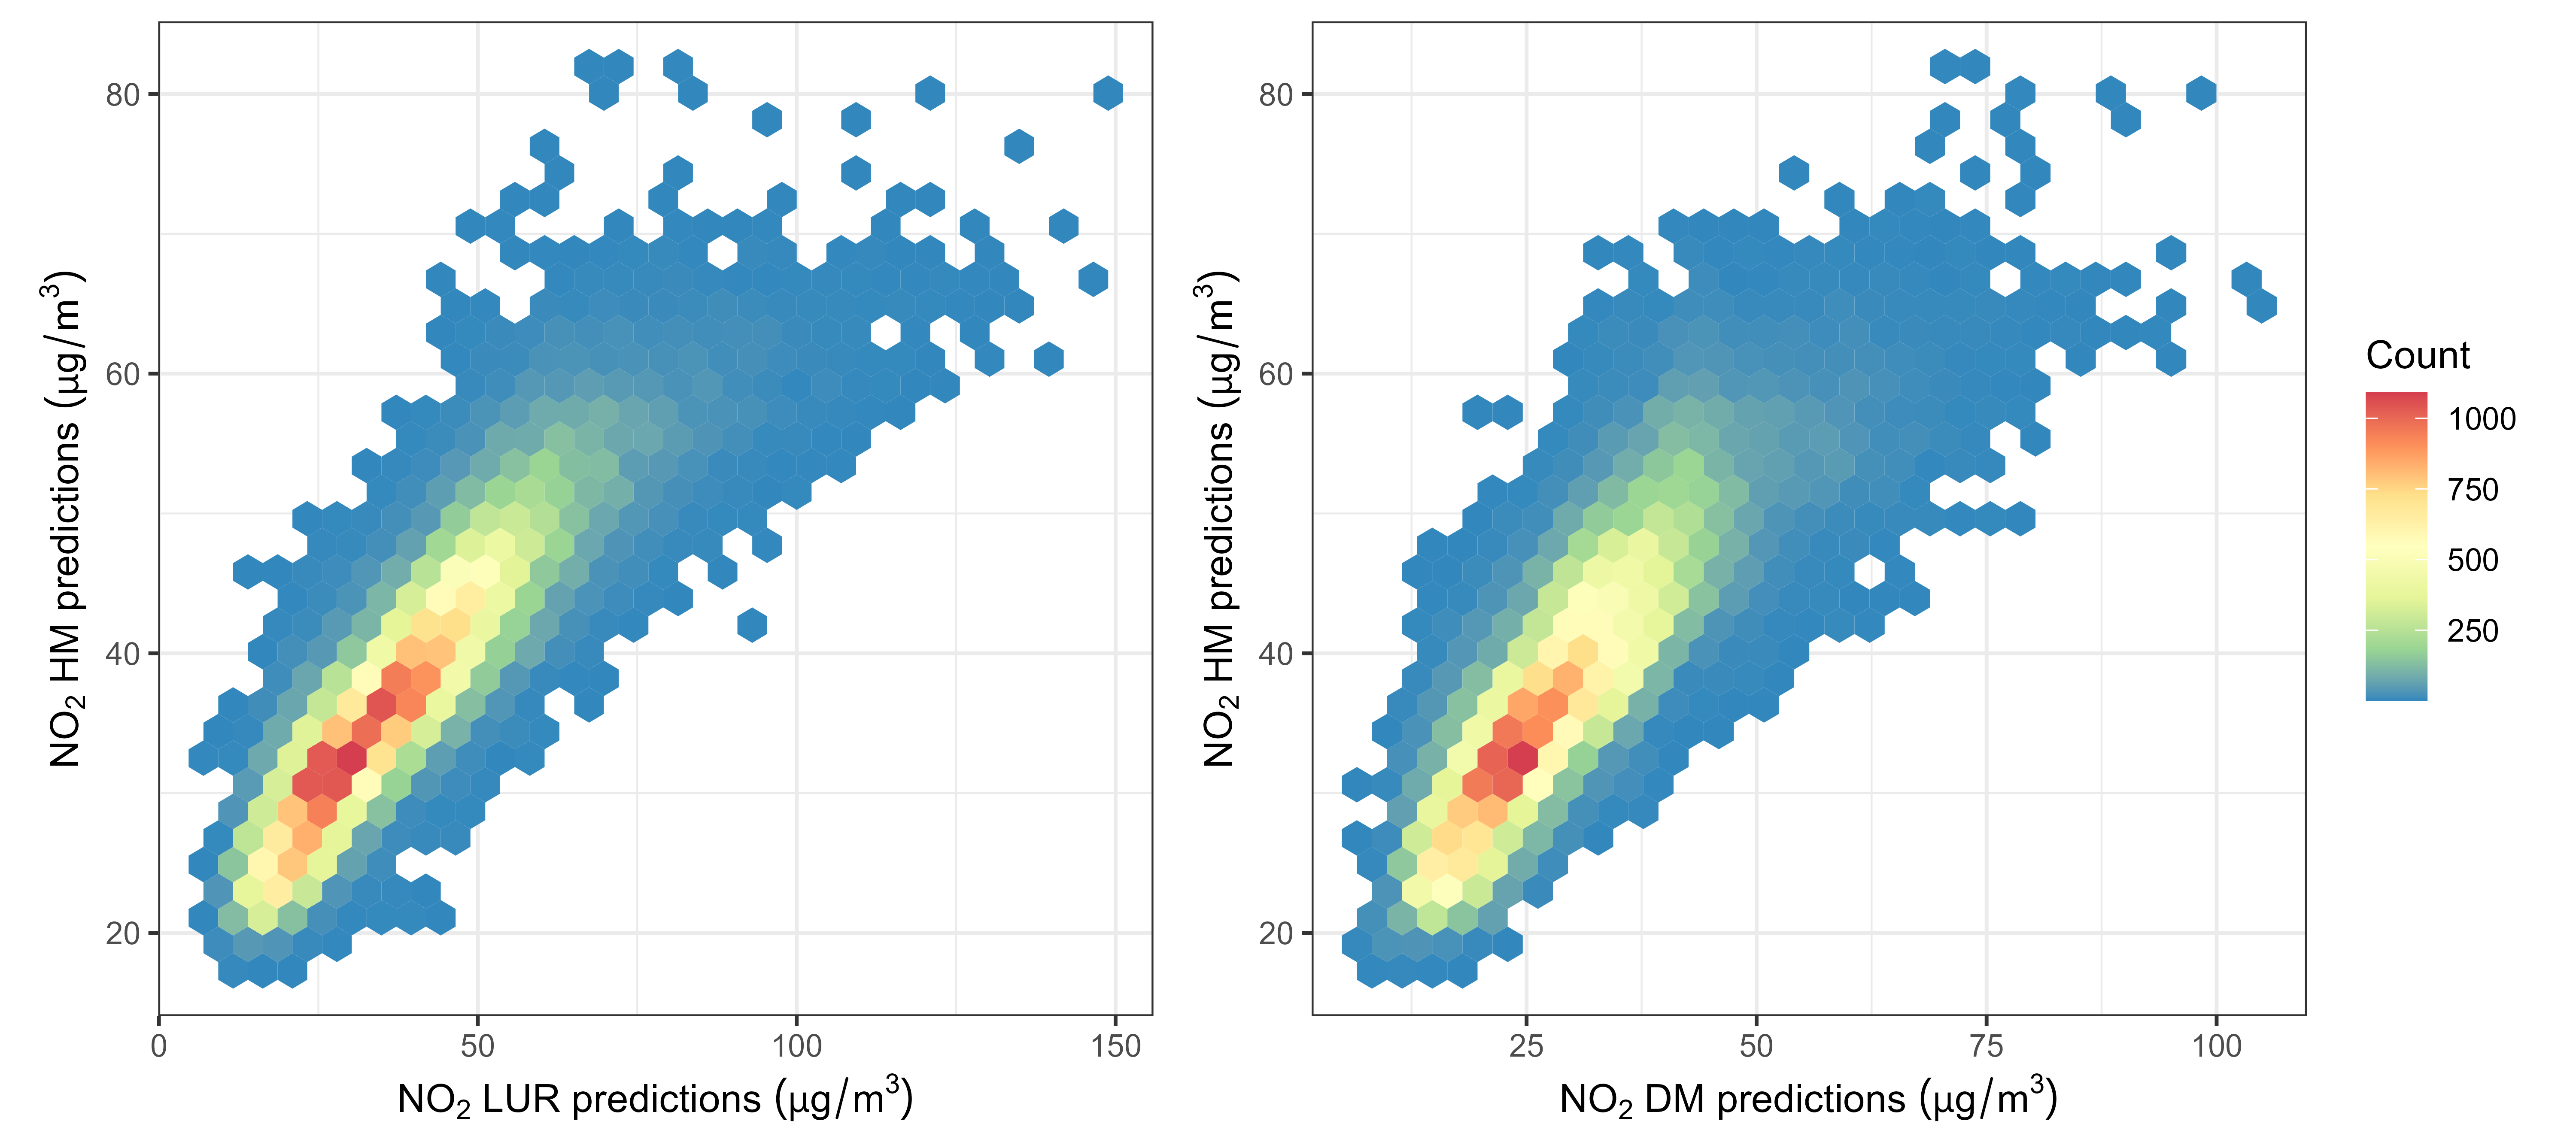
\includegraphics[width=1.0\textwidth]{figures/NO2_HEX.png}
\end{figure}

% Put the figure text closer to the Figure 3
\captionsetup[figure]{skip=6pt}
% We add the figure with the study domain 
\begin{figure}[!htb]
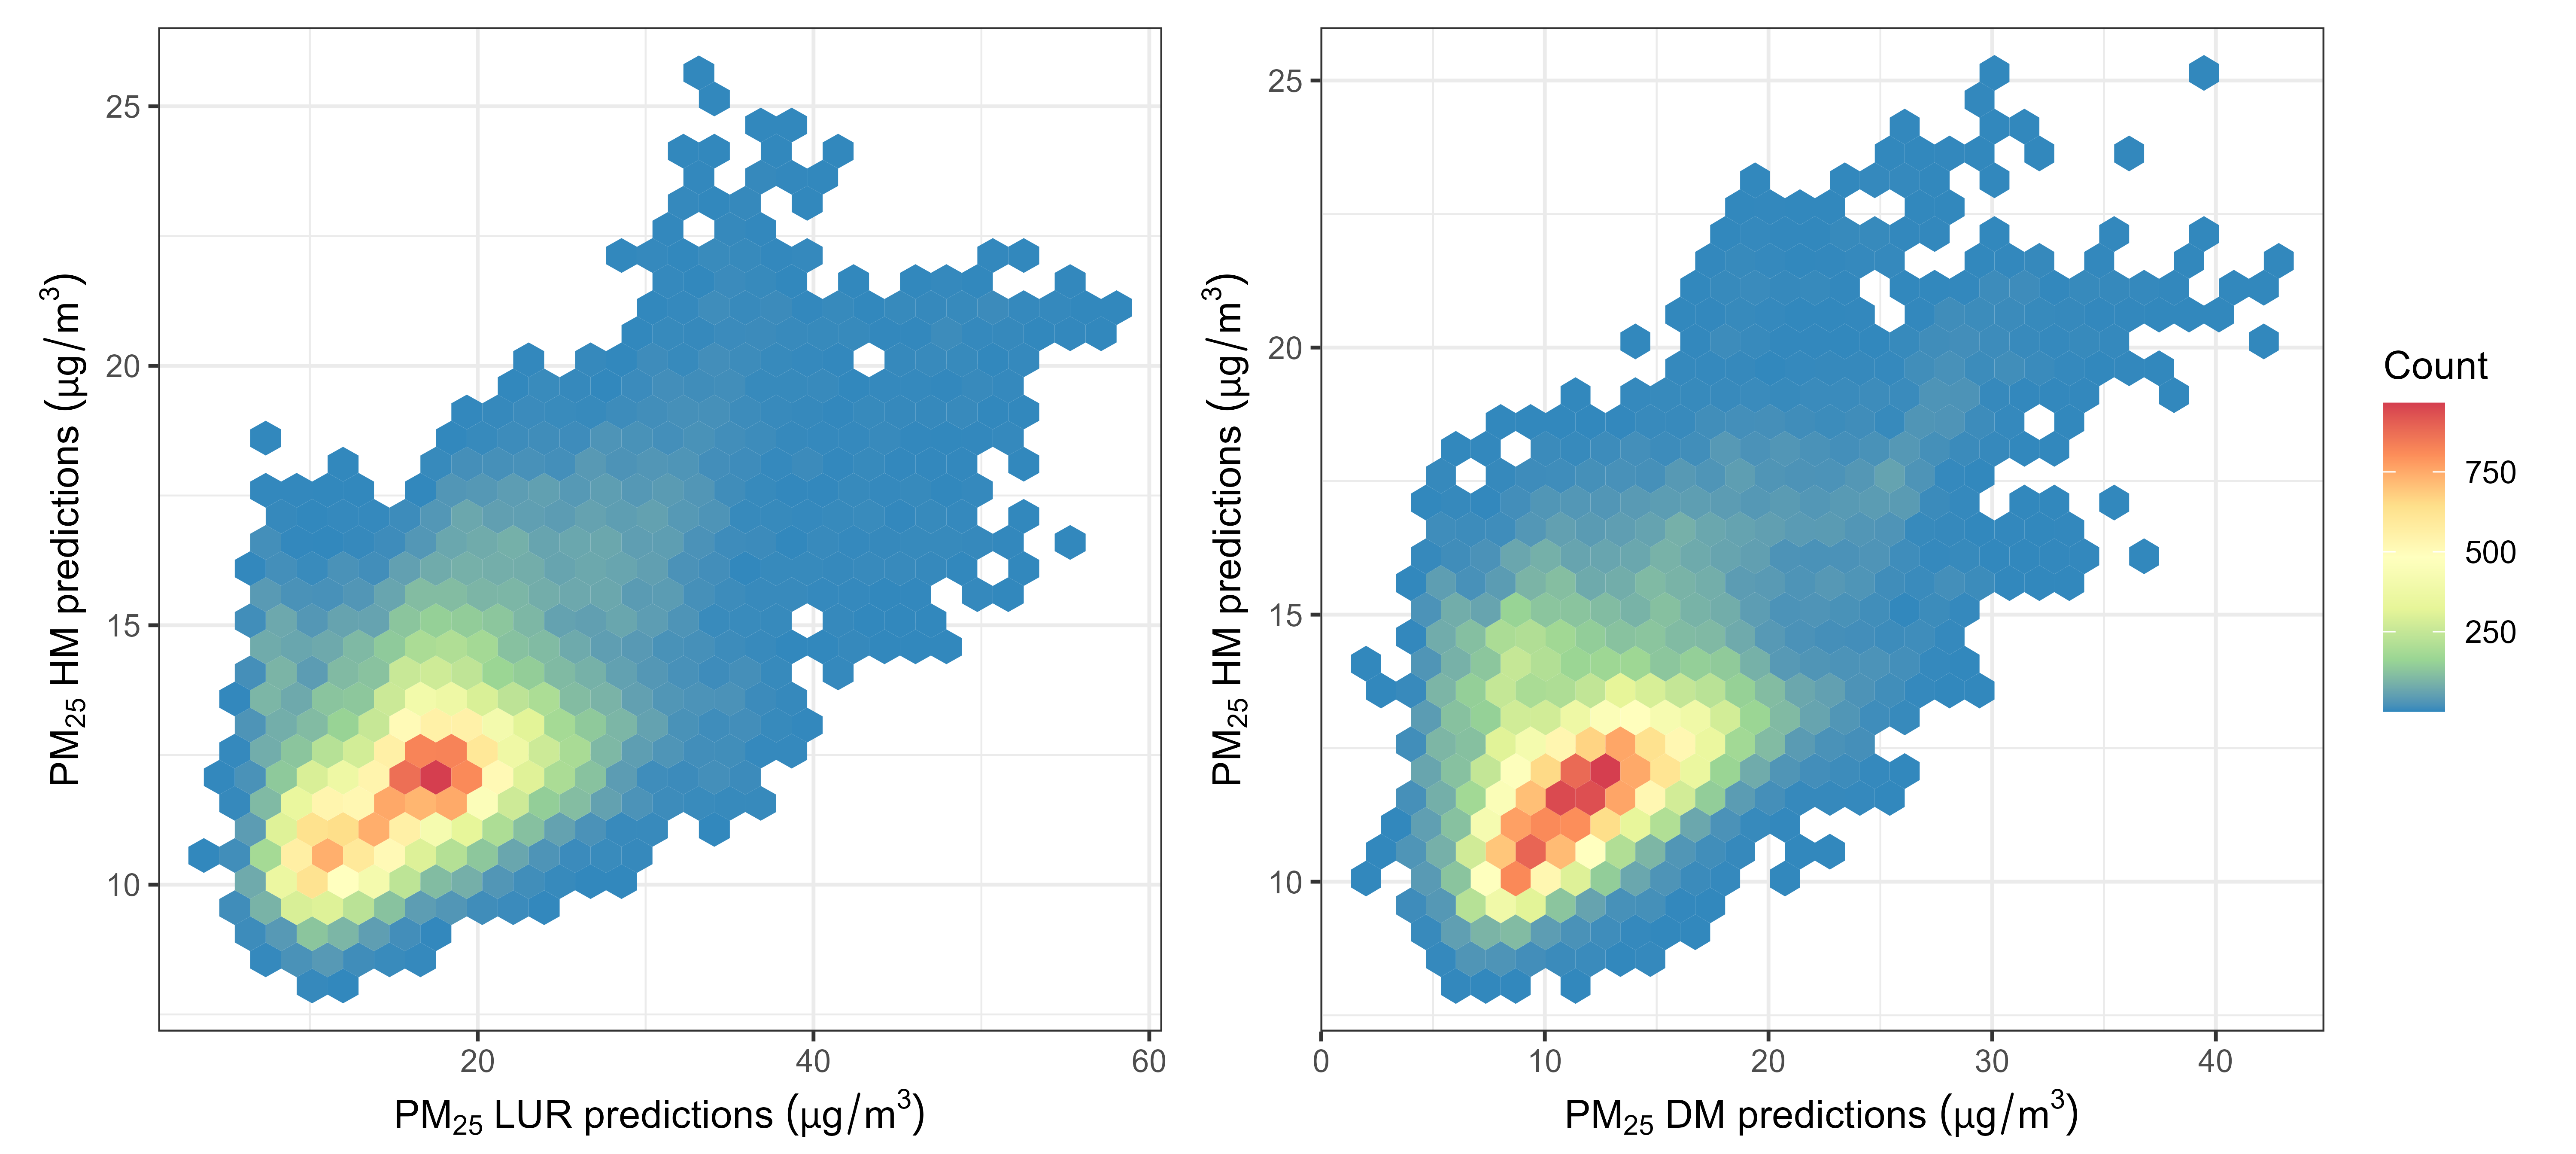
\includegraphics[width=1.0\textwidth]{figures/PM25_HEX.png}
\end{figure}

% Put the figure text closer to the Figure 3
\captionsetup[figure]{skip=6pt}
% We add the figure with the study domain 
\begin{figure}[!htb]
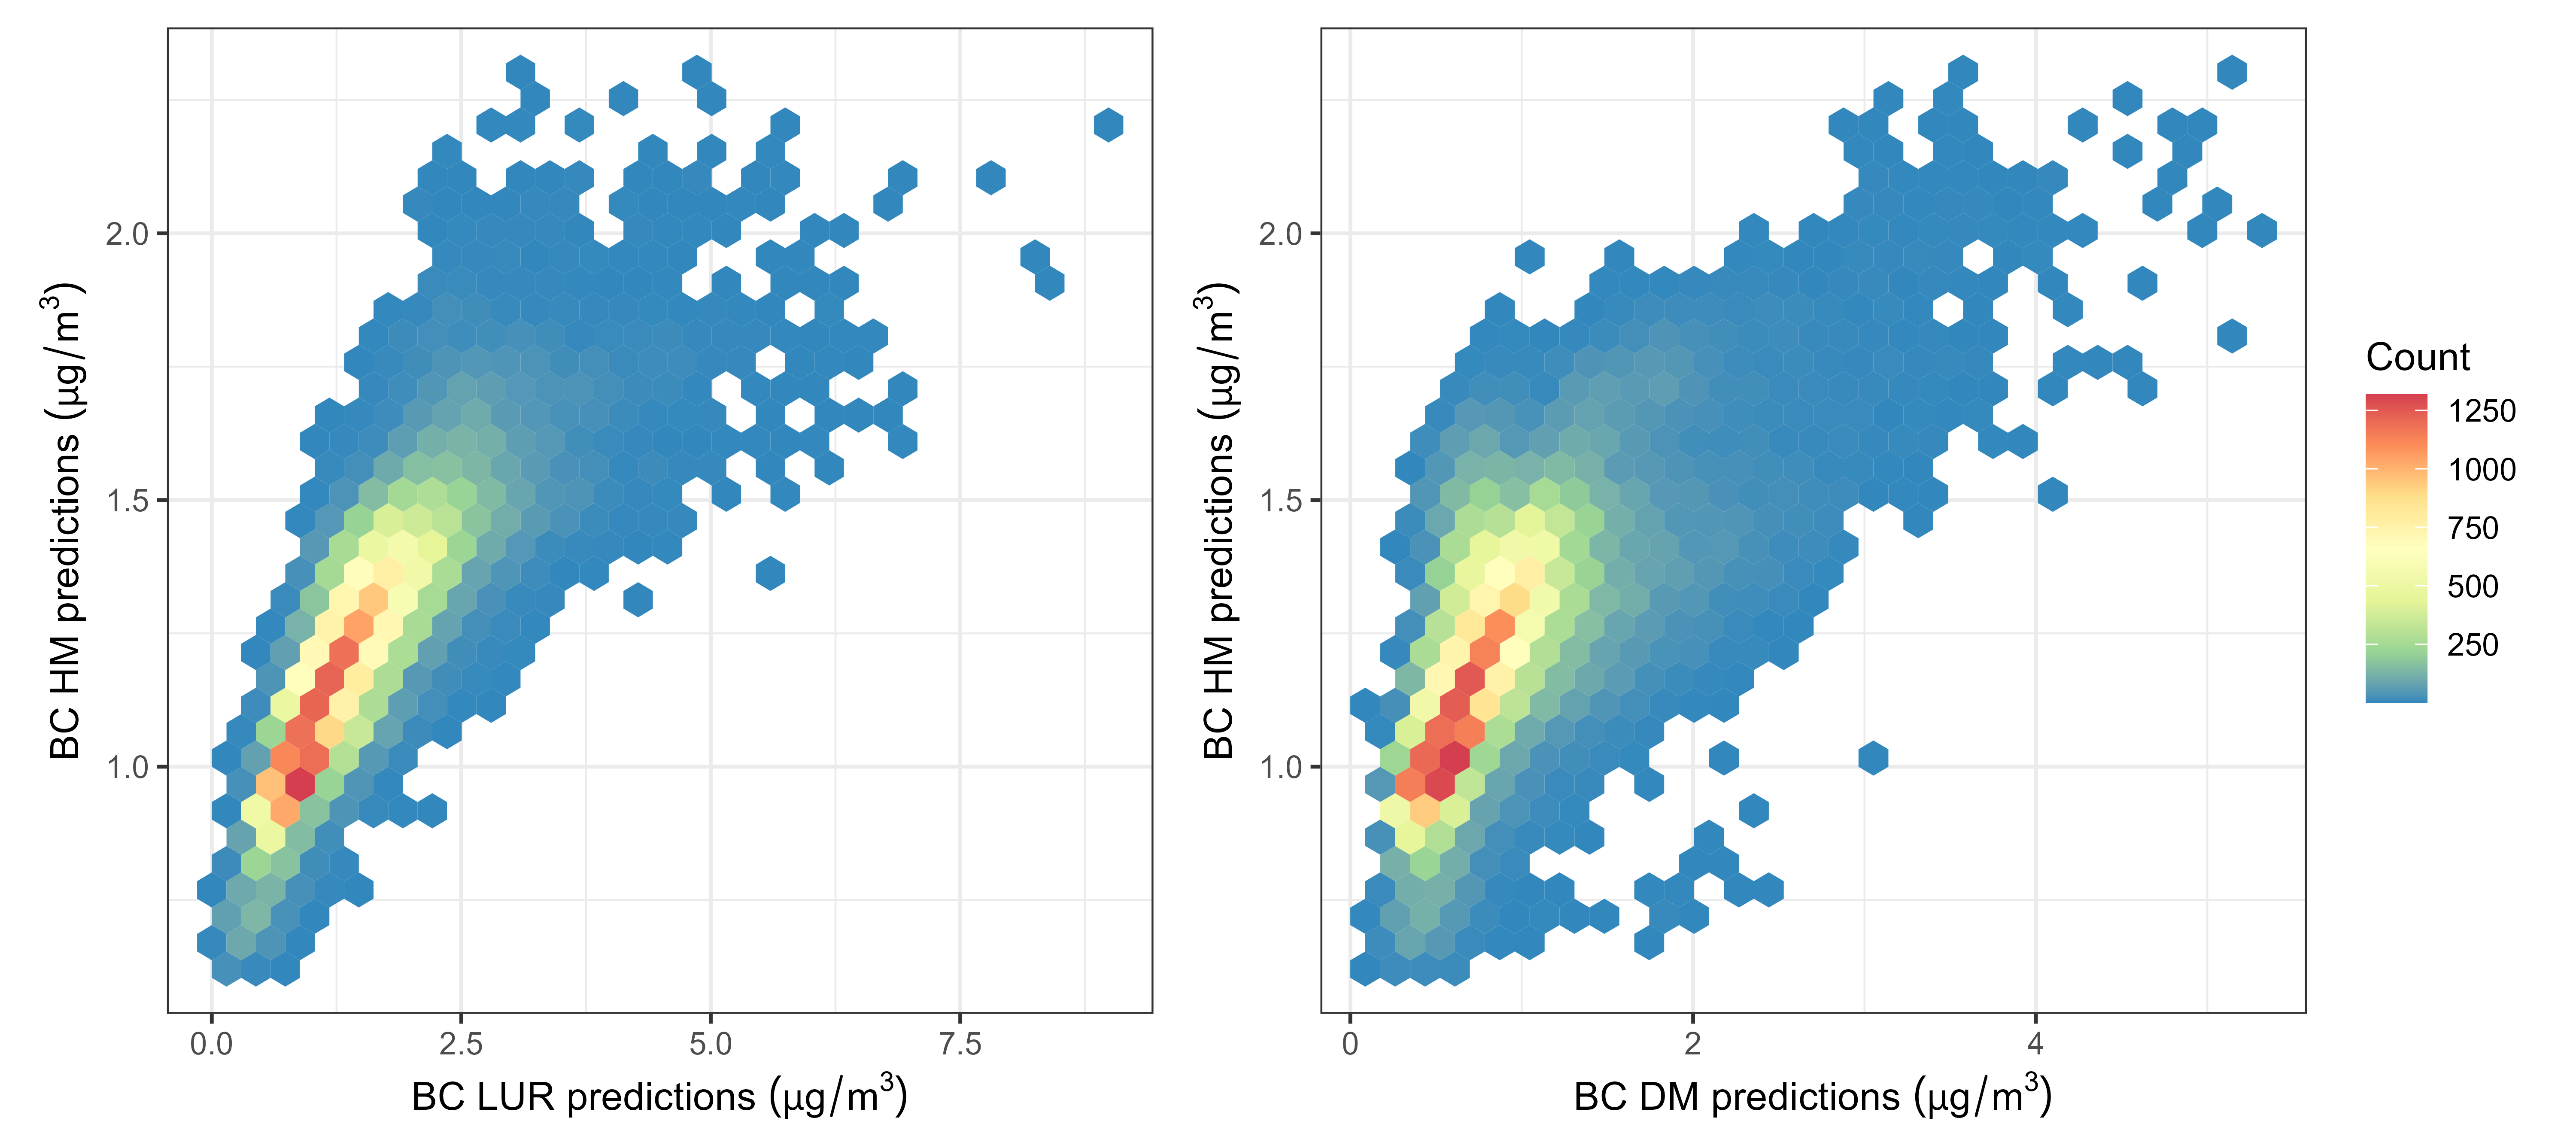
\includegraphics[width=1.0\textwidth]{figures/BC_HEX.png}
\caption{Comparison/agreement between outdoor air pollution model estimates \textit{NO$_2$}, \textit{PM$_{2.5}$}, \textit{BC}.}
\end{figure}

\newpage
%%%%%%%%%%%%%%%%%%%%%%%%%%%
%%% --- Discussion --- %%%
%%%%%%%%%%%%%%%%%%%%%%%%%
\section{Discussion}
We successfully developed spatiotemporal models using three different approaches (LUR, DM, and HM). Models show moderate to good performance 



spatiotemporal models using three different approaches (LUR, DM and HM). All models show moderate to good performance evaluated by the defined metrics in the \textbf{methods section} and displayed in more detail in the \textbf{Supplementary materials}. 

As we expected, hybrid models outperformed the LUR and DM models for the air pollutants assessed. We believe that by combining multiple data sources, and integrating RF algorithm, we were able to capture non-linear and interactions between variables and consequently improve model predictive ability. 

\subsection{Comparison between LUR, DM, and Hybrid model}






\subsection{Comparison with Previous studies}




\subsection{Strengths and Limitations}
One of the main strengths of this study is the extensive exposure assessment 

%%%%%%%%%%%%%%%%%%%%%%%%%%%
%%% --- Conclusions --- %%%
%%%%%%%%%%%%%%%%%%%%%%%%%%
\section{Conclusions}

Air pollution exposure concentration estimates from LUR, dispersion and hybrid models were moderately to strongly correlated. We observed 




%%%%%%%%%%%%%%%%%%%%%%%%%%%%%































%%%%%%%%%%%%%%%%%%%%%%%%%%%
%%% --- References --- %%%
%%%%%%%%%%%%%%%%%%%%%%%%%%%
\newpage

\bibliography{references}



\end{document}


